%\section{Software-Defined Networks: a bottom-up approach}
\section{Software-Defined Networks: Bottom-up}
\label{sec:layeredapproach}

An SDN architecture can be depicted as a composition of different layers, 
as shown in Figure~\ref{fig:sdnlayers}~(b). Each layer has its own specific functions.
While some of them are always present in an SDN deployment, such as the southbound API, 
network operating systems, northbound API and management applications, others may be 
present only in particular deployments, such as hypervisor- or language-based virtualization.

\begin{figure*}[ht!]
\centering
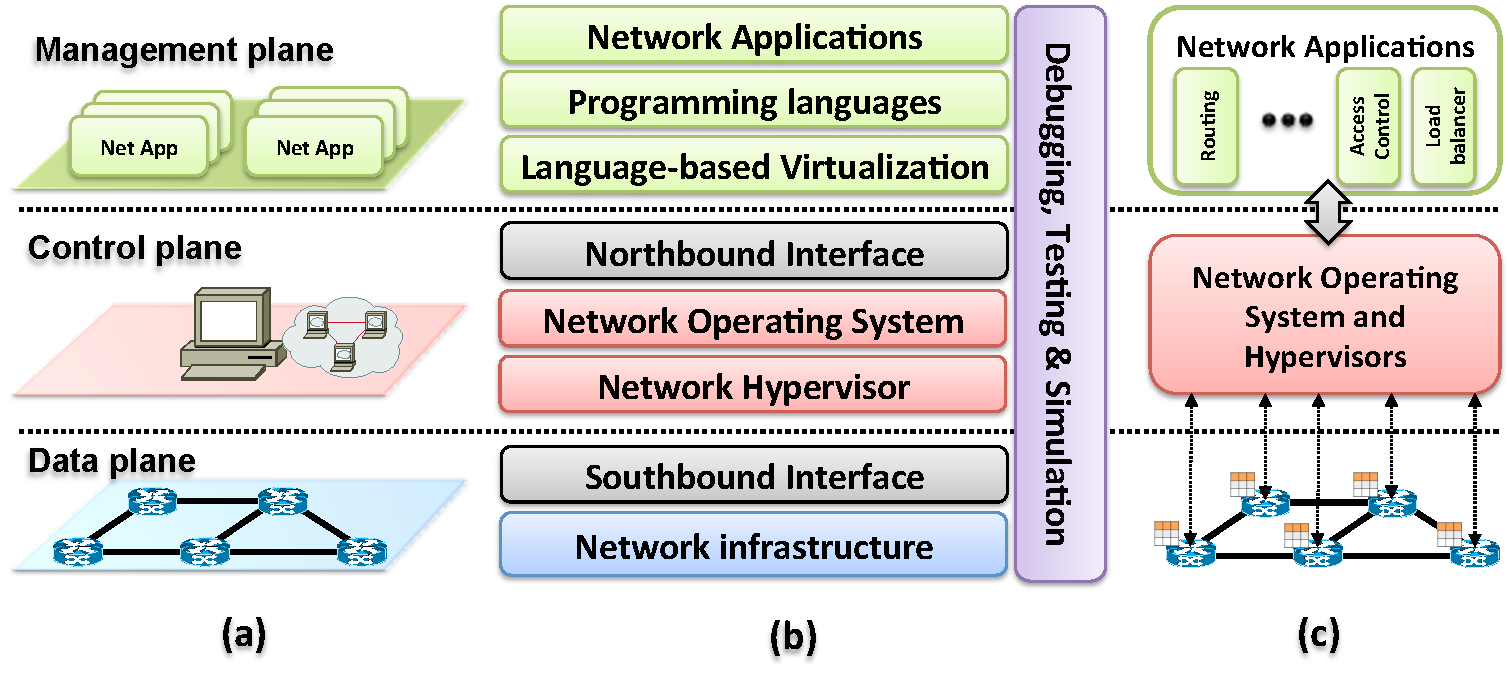
\includegraphics[width=0.85\textwidth]{figures/fig5_sdn_in_layers.pdf}
\caption{Software-Defined Networks in (a) planes, (b) layers, and (c) system design architecture}
\label{fig:sdnlayers}
\end{figure*}

Figure~\ref{fig:sdnlayers} presents a tri-fold perspective of SDNs. The SDN layers are represented 
in the center (b) of the figure, as explained above. Figures~\ref{fig:sdnlayers} (a) and ~\ref{fig:sdnlayers} (c) depict
a plane-oriented view and a system design perspective, respectively.

The following sections introduce each layer, following a bottom-up approach. For each layer, the core properties and concepts are explained based on the different technologies and solutions.  Additionally, debugging and troubleshooting techniques and tools are discussed.

\subsection{Layer I: Infrastructure}
\label{sec:infrastructure}

An SDN infrastructure, similarly to a traditional network, is composed of a set of networking 
equipment (switches, routers and middlebox appliances). The main difference resides in 
the fact that those traditional physical devices are now simple forwarding elements 
without embedded control or software to take autonomous decisions. The network intelligence is 
removed from the data plane devices to a logically-centralized control system, i.e., the network 
operating system and applications, as shown in Figure ~\ref{fig:sdnlayers} (c).
More importantly, these new networks are built (conceptually) on top of open and standard 
interfaces (e.g., OpenFlow), a crucial approach for ensuring  configuration and communication 
compatibility and interoperability among different data and control plane devices. In other words, 
these open interfaces enable controller entities to dynamically program heterogeneous forwarding 
devices, something difficult in traditional networks, due to the large variety of 
proprietary and closed interfaces and the distributed nature of the control plane.

In an SDN/OpenFlow architecture, there are two main elements, the controllers and the forwarding 
devices, as shown in Figure~\ref{fig:sdnopenflowswitch}. A data plane device is a hardware or software 
element specialized in packet forwarding, while a controller is a software stack (the ``network brain'') 
running on a commodity hardware platform. An OpenFlow-enabled forwarding device is based on a pipeline of 
flow tables where each entry of a flow table has three parts: (1) a matching rule, (2) actions to be executed 
on matching packets, and (3) counters that keep statistics of matching packets. This high-level and simplified model derived from OpenFlow is currently  the most widespread design of SDN data plane devices. Nevertheless, other specifications of SDN-enabled forwarding devices are being pursued, including POF~\cite{song2013,song2013-1} and the  Negotiable Datapath Models (NDMs) from the ONF Forwarding Abstractions Working Group (FAWG)~\cite{onf2013}.

\begin{figure*}[ht!]
\centering
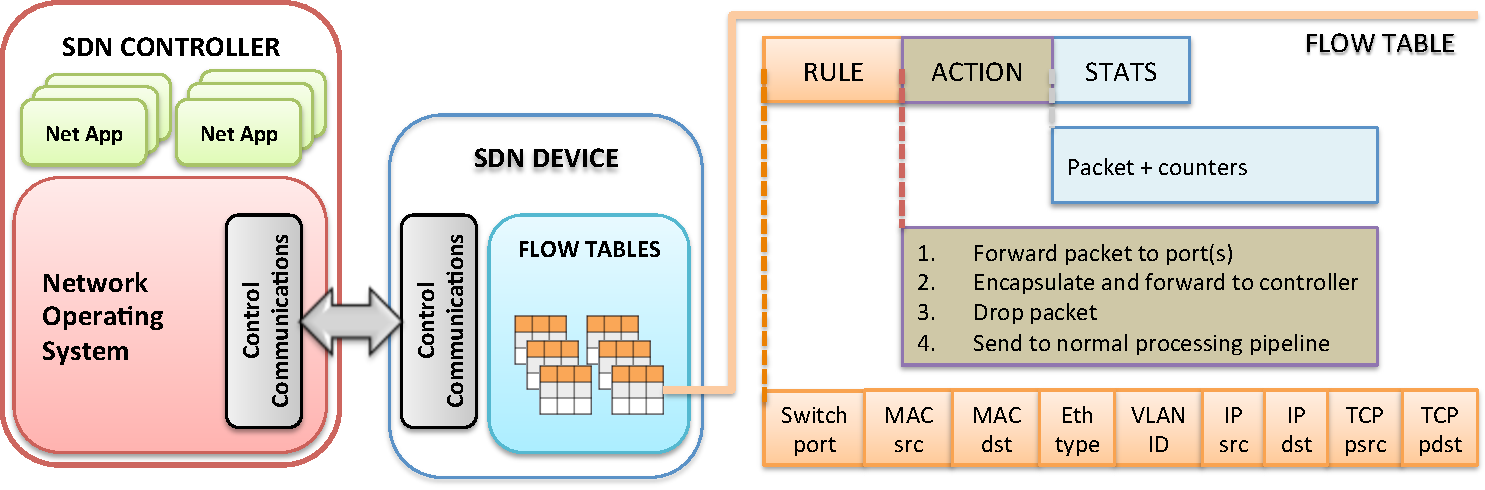
\includegraphics[width=0.85\textwidth]{figures/fig6_sdn_devices_openflow.pdf}
\caption{OpenFlow-enabled SDN devices}
\label{fig:sdnopenflowswitch}
\end{figure*}

Inside an OpenFlow device, a path through a sequence of flow tables defines how packets should be handled. 
When a new packet arrives, the lookup process starts in the first table and ends either with a match in one of the tables of the pipeline 
or with a miss (when no rule is found for that packet). 
A flow rule can be defined by combining different matching fields, as illustrated in Figure~\ref{fig:sdnopenflowswitch}.
If there is no default 
rule, the packet will be discarded. However, the common case is to install a default rule which tells the switch to send the packet to the controller (or to the normal non-OpenFlow pipeline of the switch). The priority  of the rules follows the natural sequence number of the tables and the row order in a 
flow table. Possible actions include (1) forward the packet to outgoing port(s), (2) 
encapsulate it and forward it to the controller, (3) drop it, (4) send it to the 
normal processing pipeline, (5) send it to the next flow table or to special tables, such as group or metering tables introduced in the latest OpenFlow protocol.
% versions 1.1 and 1.3, respectively.

As detailed in Table~\ref{tab:of-versions}, each version of the OpenFlow specification introduced new match fields including Ethernet, IPv4/v6, MPLS, TCP/UDP, etc. However, only a subset of those matching fields are mandatory to be compliant to a given protocol version. Similarly, many actions and port types are optional features. 
Flow match rules can be based on almost arbitrary combinations of bits of the different packet headers using bit masks for each field. Adding new matching fields has been eased with the extensibility capabilities introduced in OpenFlow version 1.2 through an OpenFlow Extensible Match (OXM) based on type-length-value (TLV) structures. To improve the overall protocol extensibility, with OpenFlow version 1.4 TLV structures have been also added to  ports, tables, and queues in replacement of the hard-coded counterparts of earlier protocol versions. 
%This provides flexibility and allows new addressing schemes on OpenFlow-enabled 
%networks, a fact that can arguably foster the development and experimentation of new 
%networking architectures and protocols, such as information and content centric networks~\cite{xxx-sdn-icn-ccn}.


{\renewcommand{\arraystretch}{1.4}
\begin{table*}[ht!]
\caption{Different match fields, statistics and capabilities have been added on each OpenFlow protocol revision. The number of required (Req) and optional (Opt) capabilities has grown considerably.}
\label{tab:of-versions}
\begin{center}
\footnotesize
\begin{tabular}{|c|l|l|c|c|c|c|c|c|c|c|}
\hline
\multirow{2}{*}{\textbf{OpenFlow Version}}        & \multirow{2}{*}{\textbf{Match fields}}           & \multirow{2}{*}{\textbf{Statistics}} & \multicolumn{2}{l|}{\textbf{\# Matches}}           & \multicolumn{2}{l|}{\textbf{\# Instructions}}    & \multicolumn{2}{l|}{\textbf{\# Actions}}          & \multicolumn{2}{l|}{\textbf{\# Ports}}           \\ \cline{4-11} 
                         &                                         &                             & Req                 & Opt                 & Req                & Opt                & Req                & Opt                 & Req                & Opt                \\ \hline  \hline
\multirow{4}{*}{v 1.0} & Ingress Port                            & Per table statistics        & \multirow{4}{*}{18} & \multirow{4}{*}{2}  & \multirow{4}{*}{1} & \multirow{4}{*}{0} & \multirow{4}{*}{2} & \multirow{4}{*}{11} & \multirow{4}{*}{6} & \multirow{4}{*}{2} \\ \cline{2-3}
                         & Ethernet: src, dst, type, VLAN                & Per flow statistics         &                     &                     &                    &                    &                    &                     &                    &                    \\ \cline{2-3}
                         & IPv4: src, dst, proto, ToS              & Per port statistics         &                     &                     &                    &                    &                    &                     &                    &                    \\ \cline{2-3}
                         & TCP/UDP: src port, dst port             & Per queue statistics        &                     &                     &                    &                    &                    &                     &                    &                    \\ \hline
\multirow{2}{*}{v 1.1} & Metadata, SCTP,  VLAN tagging       & Group statistics            & \multirow{2}{*}{23} & \multirow{2}{*}{2}  & \multirow{2}{*}{0} & \multirow{2}{*}{0} & \multirow{2}{*}{3} & \multirow{2}{*}{28} & \multirow{2}{*}{5} & \multirow{2}{*}{3} \\ \cline{2-3}
                         & MPLS: label, traffic class              & Action bucket statistics    &                     &                     &                    &                    &                    &                     &                    &                    \\ \hline
\multirow{2}{*}{v 1.2} & OpenFlow Extensible Match (OXM)         &                             & \multirow{2}{*}{14} & \multirow{2}{*}{18} & \multirow{2}{*}{2} & \multirow{2}{*}{3} & \multirow{2}{*}{2} & \multirow{2}{*}{49} & \multirow{2}{*}{5} & \multirow{2}{*}{3} \\ \cline{2-3}
                         & IPv6: src, dst, flow label, ICMPv6      &                             &                     &                     &                    &                    &                    &                     &                    &                    \\ \hline
\multirow{2}{*}{v 1.3} & \multirow{2}{*}{PBB, IPv6 Extension Headers} & Per-flow meter              & \multirow{2}{*}{14} & \multirow{2}{*}{26} & \multirow{2}{*}{2} & \multirow{2}{*}{4} & \multirow{2}{*}{2} & \multirow{2}{*}{56} & \multirow{2}{*}{5} & \multirow{2}{*}{3} \\ \cline{3-3}
                         &                                         & Per-flow meter band         &                     &                     &                    &                    &                    &                     &                    &                    \\ \hline
\multirow{2}{*}{v 1.4} & \multirow{2}{*}{---} & ---            & \multirow{2}{*}{\textbf{14}} & \multirow{2}{*}{\textbf{27}} & \multirow{2}{*}{\textbf{2}} & \multirow{2}{*}{\textbf{4}} & \multirow{2}{*}{\textbf{2}} & \multirow{2}{*}{\textbf{57}} & \multirow{2}{*}{\textbf{5}} & \multirow{2}{*}{\textbf{3}} \\ \cline{3-3}
                         &                                         & Optical port properties        &                     &                     &                    &                    &                    &                     &                    &                    \\ \hline
\end{tabular}
\end{center}
\end{table*}
}

%\vspace{2mm}
%\noindent \textit{More on OpenFlow devices}
%
%OpenFlow devices have a flow table that is configured by an external controller.
%Flow table entries are represented by rules consisting of a pattern and an action.
%A pattern can be any sequence of bits on the packet header.
%There is no strict definition of a specific address space like in IP networks, for instance.
%Additionally, rules have also an expiration time (timeout) and associated counters.
%Timeouts can be used to autonomously (by the switch itself) remove a rule from the flow table without requiring any interaction with a controller.
%There are several counters defined in the OpenFlow specification~\cite{theopennetworkingfoundation2012}.
%They can be used to collect diverse statistics from networking devices in a per flow basis.
%
%Rules can also have different granularity levels for matching the incoming flows.
%At the lowest level, a micro flow rule will match on all fields of the incoming packets.
%On the opposite side, a macro flow rule (or wildcard) can suppress (avoid matching) any number of bits in some fields.
%Therefore, it is up to the operator to define the required level of granularity.
%For instance, applications can use more than one level of granularity to solve different kinds of problems.
%While wildcards can be applied for an initial macro load balancing of incoming requests, micro flow rules may be needed to keep ongoing connection or to do finer traffic engineering when bottlenecks are close to happening.

\vspace{2mm}
\noindent \textit{Overview of available OpenFlow devices}

%At the date of this writing, 
Several OpenFlow-enabled forwarding devices are available on 
the market, both as commercial and open source products (see Table~\ref{tab:openflowdevices}).
There are many off-the-shelf, ready to deploy, OpenFlow switches and routers, among other appliances.
%A more complete list of commercially available products can be found at ~\cite{sdncentral2013}.
%Moreover, many companies have already announced new OpenFlow products~\cite{sdncentralcommunity2013}.
Most of the switches available on the market have relatively small Ternary Content-Addressable Memory (TCAMs), with up to 8K entries. 
Nonetheless, this is changing at a fast pace. Some of the latest devices released in the market go 
far beyond that figure. Gigabit Ethernet switches for common business purposes are already supporting up 
to 32K L2+L3 or 64K L2/L3 exact match flows~\cite{centecnetworks2013-1}. Enterprise class 10GE switches 
are being delivered with more than 80K Layer 2 flow entries~\cite{nec2013-1}. Other switching 
devices using high performance chips such as the EZchip NP-4, provide optimized TCAM memory that 
already supports from 125K up to 1000K flow table entries~\cite{noviflow2013-1}. This is a clear sign that the size 
of the flow tables is growing at a pace aiming to meet the needs of future SDN deployments.

Networking hardware manufacturers have produced various kinds of OpenFlow-enabled devices, as is shown in Table~\ref{tab:openflowdevices}. 
These devices range from equipment for small businesses (e.g., Gigabit Ethernet switches) to high-class data center equipment (e.g., high-density switch chassis with up to 100GbE connectivity for edge-to-core applications, with tens of Tbps of switching capacity).

{\renewcommand{\arraystretch}{1.4}
\begin{table*}[!htp]
\caption{OpenFlow enabled hardware and software devices}
\label{tab:openflowdevices}
\begin{center}
\footnotesize
%\rowcolors{1}{lightgray}{white}
\begin{tabularx}{\linewidth}{p{1.2cm}p{3.1cm}p{0.9cm}p{2.4cm}p{0.8cm}X}
\hline
\textbf{Group} & \textbf{Product} & \textbf{Type} & \textbf{Maker/Developer} & \textbf{Version} & \textbf{Short description} \\
\hline
\multirow{16}{*}{Hardware} 
& 8200zl and 5400zl~\cite{hp2013} & chassis & Hewlett-Packard & v1.0 & Data center class chassis (switch modules). \\\cline{2-6}
& Arista 7150 Series~\cite{aristanetworks2013} & switch & Arista Networks & v1.0 & Data centers hybrid Ethernet/OpenFlow switches. \\\cline{2-6}
& BlackDiamond X8~\cite{extremenetworks2013} & switch & Extreme Networks & v1.0 & Cloud-scale  hybrid Ethernet/OpenFlow switches. \\\cline{2-6}
& CX600 Series~\cite{co.2013} & router & Huawei & v1.0 & Carrier class MAN routers. \\\cline{2-6}
& EX9200 Ethernet~\cite{junipernetworks2013} & chassis & Juniper & v1.0 & Chassis based switches for cloud data centers. \\\cline{2-6}
& EZchip NP-4~\cite{yokneam2011} & chip & EZchip Technologies & v1.1 & High performance 100-Gigabit network processors. \\\cline{2-6}
& MLX Series~\cite{brocade2013} & router & Brocade & v1.0 & Service providers and enterprise class routers. \\\cline{2-6}
& NoviSwitch 1248~\cite{noviflow2013-1} & switch & NoviFlow & v1.3& High performance OpenFlow switch. \\\cline{2-6}
& NetFPGA~\cite{netfpga2014} & card & NetFPGA & v1.0 & 1G and 10G OpenFlow implementations. \\\cline{2-6}
& RackSwitch G8264~\cite{ibm2013} & switch & IBM & v1.0 & Data center switches supporting Virtual Fabric and OpenFlow. \\\cline{2-6}
& PF5240 and PF5820~\cite{nec2013-2} & switch & NEC & v1.0 & Enterprise class hybrid Ethernet/OpenFlow switches. \\\cline{2-6}
& Pica8 3920~\cite{pica8opennetworking2013} & switch & Pica8 & v1.0 & Hybrid Ethernet/OpenFlow switches. \\\cline{2-6}
& Plexxi Switch 1~\cite{plexxi2013} & switch & Plexxi & v1.0 & Optical multiplexing interconnect for data centers. \\\cline{2-6}
& V330 Series~\cite{centecnetworks2013} & switch & Centec Networks & v1.0 & Hybrid Ethernet/OpenFlow switches. \\\cline{2-6}
& Z-Series~\cite{cyan2013} & switch & Cyan & v1.0 & Family of packet-optical transport platforms.\\
\hline
\multirow{9}{*}{Software} 
& contrail-vrouter~\cite{networks2013} & vrouter &  Juniper Networks & v1.0 & Data-plane function to interface with a VRF.\\\cline{2-6}
& LINC~\cite{flowforwarding2013,rutka2013} & switch &  FlowForwarding & v1.3 & Erlang-based soft switch with OF-Config 1.1 support.\\\cline{2-6}
& ofsoftswitch13~\cite{cpqd2013} & switch & Ericsson, CPqD & v1.3 & OF 1.3 compatible user-space software switch implementation. \\\cline{2-6}
& Open vSwitch~\cite{listofcontributors2013,pfaff2009} & switch & Open Community & v1.0  & Switch platform designed for virtualized server environments.  \\\cline{2-6}
& OpenFlow Reference~\cite{openflowcommunity2009} & switch & Stanford & v1.0 & OF Switching capability to a Linux PC with multiple NICs. \\\cline{2-6}
& OpenFlowClick~\cite{mundada2009} & vrouter & Yogesh Mundada & v1.0 & OpenFlow switching element for Click software routers.\\\cline{2-6}
& Switch Light~\cite{bigswitchnetworks2013} & switch & Big Switch & v1.0  & Thin switching software platform for physical/virtual switches. \\\cline{2-6}
& Pantou/OpenWRT~\cite{yiakoumis2011} & switch & Stanford  & v1.0 & Turns a wireless router into an OF-enabled switch. \\\cline{2-6}
& XorPlus~\cite{shang2014} & switch &  Pica8 & v1.0 & Switching software for high performance ASICs.\\
\hline
\end{tabularx}
\end{center}
\end{table*}
}
%& Pica8~\cite{pica8opennetworking2013-1} & switch & Pica8 & v1.2 & Hardware independent software stack for open switches. \\\cline{2-6}
%& Indigo~\cite{projectfloodlight2013} & switch & Big Switch & v1.0 & Uses hardware features of Ethernet switch ASICs to run OF. \\\cline{2-6}
%& RouteFlow~\cite{nascimento2011} & router & CPqD & v1.0 & Virtual OpenFlow enabled routers for Internet service providers.

Software switches are emerging as one of the most promising 
solutions for data centers and virtualized network infrastructures~\cite{weissberger2013,schenker2013,casado2013}.
Examples of software-based OpenFlow switch implementations include Switch Light~\cite{bigswitchnetworks2013}, ofsoftswitch13~\cite{cpqd2013}, Open vSwitch~\cite{listofcontributors2013}, OpenFlow Reference~\cite{openflowcommunity2009}, Pica8~\cite{pica8opennetworking2013-1}, Pantou~\cite{yiakoumis2011}, and XorPlus~\cite{shang2014}.
Recent reports show that the number of virtual access ports is already larger than physical access ports on data centers~\cite{casado2013}. 
Network virtualization has been one of the drivers behind this trend.
Software switches such as Open vSwitch have been used for moving network functions to the edge (with the core performing traditional IP forwarding), thus enabling network virtualization~\cite{koponen}.

An interesting observation is the number of small, start-up enterprises devoted to SDN, such as 
Big Switch, Pica8, Cyan, Plexxi, and NoviFlow. This seems to imply that SDN is springing a more competitive and open 
networking market, one of its original goals.
Other effects of this openness triggered by SDN include the emergence of so-called ``bare metal switches'' or ``whitebox switches'', where the software and hardware are sold separately and the end-user is free to load an operating system of its choice~\cite{onie2013}. 

%%Moreover, customers have been waiting for a long time new
%%technologies for creating new conditions to drive innovation and new
%%opportunities in the ``locked down'' network world, i.e., more less
%%inflexible network infrastructures and a %%market (hard to compete
%%in) traditionally owned and controlled by a few big companies.

\subsection{Layer II: Southbound Interfaces}
\label{sec:southboundAPIs}
% FIXME: extract and put forward the essential properties of southbound APIs

Southbound interfaces (or southbound APIs) are the connecting bridges between control and forwarding 
elements, thus being the crucial instrument for clearly separating control and data plane functionality. However, 
these APIs are still tightly tied to the forwarding elements of the underlying physical or virtual 
infrastructure.

Typically, a new switch can take two years to be ready for commercialization if built from scratch, 
with upgrade cycles that can take up to nine months. The software development for a new product can 
take from six months to one year~\cite{kato2013}. The initial investment 
is high and risky. 
As a central component of its design the southbound APIs represent one of the major barriers for the introduction 
and acceptance of any new networking technology. 
In this light, the emergence of SDN southbound API proposals such as OpenFlow~\cite{mckeown2008} is seen as welcome by many in the industry.
These standards promote interoperability, allowing the deployment of vendor-agnostic network devices. 
This has already been demonstrated by the interoperability between OpenFlow-enabled equipments from different vendors.

As of this writing, OpenFlow is the most widely accepted and deployed open southbound standard 
for SDN. It provides a common specification to implement OpenFlow-enabled forwarding devices, and for the
communication channel between data and control plane devices (e.g., switches and controllers).
%An OpenFlow-enabled switch is similar to a normal Ethernet device, except that it does not act 
%autonomously. Actually, since the OpenFlow 1.1.0 specification~\cite{onf2012}, 
%there is a standalone operation mode, which can be enabled when the connection with the controller 
%fails. In this case, the device will act exactly as an Ethernet switch. Apart from exceptional 
%situations, an OpenFlow device will look for a matching rule in the local flow tables for every 
%incoming packet. A positive match tells the device what to do with the ingress packet, i.e., which 
%actions to take.
The OpenFlow protocol provides three information sources for network operating systems.
First, event-based messages are sent by forwarding devices to the controller when a link or port 
change is triggered. Second, flow statistics are generated by the forwarding devices and collected 
by the controller. Third, packet-in messages are sent by forwarding devices to the controller when 
they do not known what to do with a new incoming flow or because there is an explicit ``send to 
controller'' action in the matched entry of the flow table. These information channels are the essential 
means to provide flow-level information to the network operating system.

Albeit the most visible, OpenFlow is not the only available southbound interface for SDN.
There are other API proposals such as ForCES~\cite{doria2010}, OVSDB~\cite{pfaff2013-1}, POF~\cite{song2013,song2013-1}, and OpFlex~\cite{smith2014}.
ForCES proposes a more flexible approach to traditional network management without changing the current architecture of the network, i.e., without the need of a logically-centralized external controller. 
The control and data planes are separated but can potentially be kept in the same network element.
However, the control part of the network element can be upgraded on-the-fly with third-party firmware.
%, for instance.

%Interestingly, despite ForCES being older than OpenFlow, it is not yet widely accepted or supported on commercial products.
%Nevertheless, this does not mean its end because we are only on the early chapters of SDN.
%There is plenty space and opportunity for new southbound APIs.
%History has shown us that different environments, requirements and market needs are some of the major driving forces for developing new technologies and solutions.

OVSDB~\cite{pfaff2013-1} is another type of southbound API, designed to provide 
advanced management capabilities for Open vSwitches. Beyond OpenFlow's capabilities to configure 
the behavior of flows in a forwarding device, an Open vSwitch offers other networking functions.
For instance, it allows the control elements to create multiple virtual switch instances, set QoS 
policies on interfaces, attach interfaces to the switches, configure tunnel interfaces on OpenFlow 
data paths, manage queues, and collect statistics.
Therefore, the OVSDB is a complementary protocol to OpenFlow for Open vSwitch. 


%OpenSketch~\cite{yu2013-1} is an example of a more specific southbound API.
%It proposes data and control plane abstractions specifically for measurement purposes.
%One of the goals of OpenSketch is to allow multiple measurement tasks to execute concurrently without impairing accuracy.
%
%The internal design of a OpenSketch switch can be seen as a pipeline with three stages (hashing, classification, counting).
%Input packets have to first pass through a hashing function.
%Then they are classified accordingly a matching rule.
%Lastly, the match rule identifies a counting index, which is used to calculate the counter location in the counting stage.
%While a TCAM with few entries is enough for stage two (classification rules), the flexible counters are stored in SRAM.
%This makes the OpenSketch's operation efficient (fast matching) and costly effectively (cheaper SRAMs to store counters).
%However, differently from OpenFlow, OpenSketch is a special purpose southbound API designed to provide flexibility for measurements.
%\note{DK: Maybe, move to another place --- monitoring, applications, etc.}

One of the first direct competitors of OpenFlow is POF~\cite{song2013,song2013-1}.
One of the main goals of POF is to enhance the current SDN forwarding plane.
With OpenFlow, switches have to understand the protocol headers to extract the required bits to be matched with the flow tables entries.
This parsing represents a significant burden for data plane devices, in particular if we consider that OpenFlow version 1.3 already contains more  than 40 header fields. 
Besides this inherent complexity, backward compatibility issues may arise every time new header fields are included in or removed from the protocol.
To achieve its goal, POF proposes a generic flow  instruction set (FIS) that makes the forwarding plane protocol-oblivious.
A forwarding element does not need to know, by itself, anything about the packet format in advance.
Forwarding devices are seen as white boxes with only processing and forwarding  capabilities. 
In POF, packet parsing is a controller task that results in a sequence of generic keys and table lookup instructions that are installed in the forwarding elements.
The behavior of data plane devices is therefore completely under the control of the SDN controller.
Similar to a CPU in a computer sytem, a POF switch is application- and protocol-agnostic. 

A very recent soutbound interface proposal is OpFlex~\cite{smith2014}.
Contrary to OpenFlow (and similar to ForCES), one of the ideas behind OpFlex is to distribute part of the 
complexity of managing the network back to the forwarding devices, with the aim of improving scalability.
Similar to OpenFlow, policies are logically centralized and abstracted from the underlying implementation.
The differences between OpenFlow and OpFlex are a clear illustration of one of the important questions to be answered when devising a southbound interface: where to place each piece of the overall functionality. 

\subsection{Layer III: Network Hypervisors}
\label{sec:virtualizationhypervisor}

Virtualization is already a consolidated technology in modern computers. The fast 
developments of the past decade have made virtualization of computing platforms mainstream.
Based on recent reports, the number of virtual servers has already exceeded the number of physical 
servers~\cite{bittman2013,koponen}.

Hypervisors enable distinct virtual machines to share the same hardware resources. In a 
cloud infrastructure-as-a-service (IaaS), each user can have its own virtual resources, from computing to 
storage. This enabled new revenue and business models where users allocate resources on-demand, from a shared 
physical infrastructures, at a relatively low cost.
% (less CAPEX and OPEX expenditures, for instance). 
At the same time, providers make better use of the capacity of their installed physical 
infrastructures, creating new revenue streams without significantly increasing their CAPEX and OPEX 
costs. One of the interesting features of virtualization technologies today is the fact that virtual 
machines can be easily migrated from one physical server to another and can 
be created and/or destroyed on-demand, enabling the provisioning of elastic services with flexible 
and easy management.
Unfortunately, virtualization has been only partially realized in practice. Despite the great advances 
in virtualizing computing and storage elements, the network is still mostly statically configured in a box-by-box manner~\cite{chowdhury2010}.

The main network requirements can be captured along two dimensions: network topology and address space.
Different workloads require different network topologies and services, such as flat L2 or L3 services, or even more complex L4-L7 
services for advanced functionality.
Currently, it is very difficult for a single physical topology to support the diverse demands 
of applications and services. Similarly, address space is hard to change in current networks. Nowadays, 
virtualized workloads have to operate in the same address of the physical infrastructure. 
Therefore, it is hard to keep the original network configuration for a tenant, virtual machines can not migrate to arbitrary locations, and the addressing scheme is fixed and hard to change. 
For example, IPv6 cannot be used by the VMs of a tenant if the underlying physical forwarding devices support only IPv4.

%It is also worth emphasizing that traditional networks have a fairly static nature and are complex to manage.
%Things such as virtualization, live network migration or network changes are yet hard to implement.
%Therefore, flexible, fast, scalable and on-demand network virtualization is still one of the major open challenges in the network world.

To provide complete virtualization the network should provide similar properties to the computing layer~\cite{chowdhury2010}.
The network infrastructure should be able to support arbitrary network topologies and addressing schemes.
Each tenant should have the ability to configure both the computing nodes and the network simultaneously.
Host migration should automatically trigger the migration of the corresponding virtual network ports.
One might think that long standing virtualization primitives such as VLANs (virtualized L2 domain), NAT (Virtualized IP address space), and 
MPLS (virtualized path) are enough to provide full and automated network virtualization.
However, these  technologies are anchored on a box-by-box basis configuration, i.e., there is no single unifying 
abstraction that can be leveraged to configure (or reconfigure) the network in a global manner.
As a consequence, current network provisioning can take months, while computing provisioning takes only 
minutes~\cite{koponen,cearley2013,peng2012,zhang2014}.

There is hope that this situation will change with SDN and the availability of new tunneling techniques (e.g., VXLAN~\cite{mahalingam2013}, NVGRE~\cite{sridharan2013}).
For instance, solutions such as FlowVisor~\cite{sherwood2009,sherwood2010,azodolmolky2012},  FlowN~\cite{drutskoy2012}, NVP~\cite{koponen}, OpenVirteX~\cite{al-shabibi2014} and IBM SDN VE~\cite{racherla2014,li2014}
have been recently proposed, evaluated and deployed in real scenarios for on-demand provisioning of virtual 
networks.

\vspace{2mm}
\noindent \textit{Slicing the network}

FlowVisor is one of the early technologies to virtualize a Software-Defined Network.
%FlowVisor is also the first known hypervisor for OpenFlow-based SDNs. 
Its basic idea is to allow multiple logical networks share the same OpenFlow networking infrastructure.
For this purpose, it provides an abstraction layer that makes it easier to slice a data plane based on off-the-shelf OpenFlow-enabled switches, allowing multiple and diverse networks to co-exist. 
%More interestingly, it works with off-the-shelf OpenFlow-enabled switches, not requiring any 
%specialized or programmable hardware such as FPGAs or specific network processors.

Five slicing dimensions are considered in FlowVisor: bandwidth, topology, traffic, device CPU and forwarding 
tables. Moreover, each network slice supports a controller, i.e., multiple controllers can co-exist on top 
of the same physical network infrastructure. Each controller is allowed to act only on its own network slice.
In general terms, a slice is defined as a particular set of flows on the data plane. 
From a system design perspective, FlowVisor is a transparent proxy that intercepts OpenFlow messages between 
switches and controllers. It partitions the link bandwidth and flow tables of each switch. Each slice receives 
a minimum data rate and each guest controller gets its own virtual flow table in the switches.

Similarly to FlowVisor, OpenVirteX~\cite{al-shabibi2014} acts as a proxy between the network operating system and the forwarding 
devices. However, its main goal is to provide virtual SDNs through both topology, address, and control function
virtualization. 
All these properties are necessary in multi-tenant environments where virtual networks 
need to be managed and migrated according to the computing and storage virtual resources. Virtual network 
topologies have to be mapped onto the underlying forwarding devices, with virtual addresses allowing tenants 
to completely manage their address space without depending on the underlying network elements addressing schemes.

AutoSlice~\cite{bozakov2012} is another SDN-based virtualization proposal. Similar to FlowVisor, the idea is to 
allow multiple controllers to manage their respective virtual SDN.
The main difference is that AutoSlice intends to develop a transparent virtualization layer, or SDN hypervisor, 
to automate the deployment of virtual SDNs in a less cumbersome manner than FlowVisor.

FlowN~\cite{drutskoy2012,drutskoy2013} is based on a slightly different concept. Whereas FlowVisor can be compared to a full virtualization technology, FlowN 
is analogous to a container-based virtualization, i.e., a lightweight virtualization approach. FlowN 
was also primarily conceived to address multi-tenancy in the context of cloud platforms. It is designed to 
be scalable and allows a unique shared controller platform to be used for managing multiple domains 
in a cloud environment. Each tenant has full control over its virtual networks and is free to deploy 
any network abstraction and application on top of the controller platform.


\vspace{2mm}
\noindent \textit{Commercial multi-tenant network hypervisors}

None of the aforementioned approaches is designed to address all challenges of multi-tenant 
data centers. For instance, tenants want to be able to migrate their enterprise solutions to cloud 
providers without the need to modify the network configuration of their home network. Existing 
networking technologies and migration strategies have mostly failed to meet both the tenant and the 
service provider requirements.
A multi-tenant environment should be anchored in a network hypervisor capable of abstracting the 
underlaying forwarding devices and physical network topology from the tenants. Moreover, each tenant 
should have access to control abstractions and manage its own virtual networks independently and 
isolated from other tenants.

With the market demand for network virtualization and the recent research on SDN showing promise as an enabling technology, different commercial virtualization platforms based on SDN concepts have started to appear.
VMWare has proposed a network virtualization platform (NVP)~\cite{koponen} that provides the necessary abstractions to allow the creation of independent virtual networks for large-scale multi-tenant environments.
NVP is a complete network virtualization solution that allows the creation of virtual networks, each with independent service model, topologies, and addressing architectures over the same physical network.
With NVP, tenants do not need to know anything about the underlying network topology, configuration or other specific aspects of the forwarding devices. 
NVP's network hypervisor translates the tenants configurations and requirements into low level instruction sets to be installed on the forwarding devices. 
For this purpose, the platform uses a cluster of SDN controllers to manipulate the forwarding tables of the Open vSwitches in the host's hypervisor. 
Forwarding decisions are therefore made exclusively on the network edge.
After the decision is made, the packet is tunneled over the physical network to the receiving host hypervisor (the physical network sees nothing but ordinary IP packets).

IBM has also recently proposed SDN VE~\cite{racherla2014,li2014}, another commercial and enterprise-class network virtualization platform.
SDN VE uses OpenDaylight as one of its building blocks for Software-Defined Environments (SDEs)\footnote{We will return to OpenDaylight and SDE later.}.
This solutions also offers a complete implementation framework for network virtualization. 
Like NVP, it uses a host-based overlay approach, achieving advanced network abstraction that enables application-level network services in large-scale multi-tenant environments. 
%It provides a multi-hypervisor, server-centric solution comprising multiple components that overlay virtual networks onto any physical network that provides IP connectivity.
Interestingly, SDN VE 1.0 is capable of supporting in one single instantiation up to 16,000 virtual networks and 128,000 virtual machines~\cite{racherla2014,li2014}.
%The overall solution is designed to support up to 16M virtual networks in a global deployment.
%distinct virtual networks for multi-tenancy separation and isolation, multicast support without needing to be supported on the underlaying %hardware.
%This gives a rough idea of what future software-defined environments will be capable of delivering for the  evolution of IT infrastructures.

To summarize, currently there are only a few network hypervisor proposals leveraging the advances of SDN.
We antecipate, however, this ecosystem to expand in the near future since network virtualization will most likely play a key role in future virtualized environments, similarly to the expansion we have been witnessing in virtualized computing.

%By providing also overlay networks for backward compatibility, SDN VE also ensures:
%scalability on  L2 and L3 independently from the underlying network infrastructure;
%reduced exposure of MAC addresses in the underlay network;
%migration capabilities across data centers using L3 without any kind of dependency on the existing underlaying L2;
%smoothly migration of workloads to any location while still retaining the physical addressing scheme, even when overlapping schemes are used;
%broadcast isolation within each DMZ; and 
%open standard integration of systems without any kind of hardware or vendor lock-in.

%As an example of its interoperability capabilities, which are embedded since its conception, SDN VE is already integrated with VMware and KVM hypervisors/technologies, as well as OpenFlow-enabled devices through the unified controller.
%Furthermore, another cornerstone of the solution is the DOVE Overlay network, which, among other things, provides backward compatibility and interoperability. 
% What is does is to create virtual networks that transparently allow VM to VM communication throughout the infrastructure, without requiring any change on existing underlay network that it rides over.
% In other words, it represents and integration for a seamless migration between current existing infrastructures and OpenFlow-enabled data planes.
% One of the key technologies used by the DOVE Overlay is the VXLAN frame format.


\subsection{Layer IV: Network Operating Systems / Controllers}
\label{sec:controllers}

Traditional operating systems provide abstractions (e.g., high-level programming APIs) for accessing 
lower-level devices, manage the concurrent access to the underlying resources (e.g., hard drive, network 
adapter, CPU, memory), and provide security protection mechanisms. These functionalities and resources 
are key enablers for increased productivity, making the life of system and application developers easier. Their 
widespread use has significantly contributed to the evolution of various ecosystems (e.g., programming 
languages) and the development of a myriad of applications.

In contrast, networks have so far been managed and configured using lower level, device-specific instruction 
sets and mostly closed proprietary network operating systems (e.g., Cisco IOS and Juniper JunOS). 
Moreover, the idea of operating systems abstracting device-specific characteristics 
and providing, in a transparent way, common functionalities is still almost absent in networks.
For instance, nowadays designers of routing protocols need to deal with complicated distributed algorithms when solving networking problems.
Network practitioners have therefore been solving the same problems over and over again.

SDN is promised to facilitate network management and ease the burden of solving networking problems by means of the logically-centralized control offered by a network operating system (NOS)~\cite{gude2008}.
As with traditional operating systems, the crucial value of a NOS is to provide abstractions, essential services, 
and common application programming interfaces (APIs) to developers. 
Generic functionality as network state and network topology information, device discovery, and distribution of network configuration can be provided as services of the NOS.
With NOSs, to define network policies a developer no longer needs to care about the low-level details of data distribution among routing elements, for instance.
Such systems can arguably create a new environment capable of fostering innovation at a faster pace by reducing the inherent complexity of creating new network protocols and management applications.

A NOS (or controller) is a critical element in an SDN architecture as it is the key supporting piece 
for the control logic (applications) to generate the network configuration based on the policies defined by the network operator. 
Similar to a traditional operating system, the control platform abstracts the lower-level details of connecting and interacting with forwarding devices (i.e., of materializing the network policies).

%\vspace{2mm}
%\noindent \textit{Inside a controller}
%
%Figure~\ref{fig:controllerarchitecture} illustrates a simplified internal architecture of a controller.
%It gives an idea of how a controller and management applications deal with requests from forwarding devices.
%Incoming requests can go simultaneously through one or more pipelines of applications.
%For instance, programming languages like Pyretic~\cite{monsanto2013} make it possible this kind of composition, allowing two distinct configurations, parallel pipelines (e.g., packets are processed at the same time by apps 3 and 4) and sequential pipelines (e.g., packets go sequentially through apps 1 and 2).
%Regardless of the set of applications and pipelines, the output is always the same, i.e., programming/configuration data or data requests to be send to the forwarding devices.
%
%\begin{figure}[ht]
%\centering
%\includegraphics[width=\columnwidth]{figures/sdn-controller-internals-v3.pdf}
%\caption{Illustrated controller internals}
%\label{fig:controllerarchitecture}
%\end{figure}
%
%However, each controller can have a specific internal architecture that depends on design, development and technology choices with its inherent constraints.
%While some controllers have flow processing pipelines and are able to handle applications in parallel, others allow only a more static and sequential combination of applications.
%Controllers are also designed to explore two kinds of parallelism, on the application level and on the flow processing capabilities.
%Therefore, in some controllers even a single application pipeline may have concurrent instances for higher throughput, for instance.
%Moreover, there are controllers that have additional mechanisms to deal with concurrency problems such as packets/requests issued by a switch for a flow that is already in a configuration process.
%These kind of requests/packets can be automatically discharged by the controller.
%
%% FIXME: look for the best place to introduce these practical aspects of OpenFlow controllers
%In practical terms, the three top features in most OpenFlow controllers are:
%\begin{enumerate}
%\item \textit{Event-driven model}: each module registers listeners or call-back functions (example of async events include PACKET\_IN, PORT\_STATUS, FEATURE\_REPLY, STATS\_REPLY).
%\item \textit{Packet parsing capabilities}: when switch sends an OpenFlow message, module extracts relevant information using standard procedures.
%\item \textit{switch.send(msg)}, where msg can be
%  \begin{itemize}
%  \item PACKET\_OUT with buffer\_id or fabricated packet
%  \item FLOW\_MOD with match rules and action taken
%  \item FEATURE\_REQUEST, STATS\_REQUEST, BARRIER\_REQUEST
%  \end{itemize}
%\end{enumerate}
%


\vspace{2mm}
\noindent \textit{Architecture and design axes}
\vspace{2mm}

%While a controller can be seen as the kernel of an operating system, a control platform can be viewed as an operating system distribution (e.g., Ubuntu Linux).
There are very diverse controllers and control platforms with different design and architectural choices~\cite{koponen-1,opendaylight2013,junipernetworks2013-1,hp2013-1,phemius2013,erickson2013-1}.
Existing controllers can be categorized based on many aspects. 
From an architectural point of view, one of the most relevant is if they are centralized or distributed.
This is one of the key design axes of SDN control platforms, so we start by discussing this aspect next. 

\vspace{2mm}
\noindent \textit{Centralized vs. Distributed}

A centralized controller  is a single entity that manages all forwarding devices of the network.
Naturally, it represents a single point of failure and may have scaling limitations.
A single controller may not be enough to manage a network with a large number of data plane elements. 
Centralized controllers such as NOX-MT ~\cite{tootoonchian2012},
Maestro~\cite{cai2011}, Beacon~\cite{erickson2013}, and Floodlight~\cite{openflowhub.org2012}    
have been designed as highly concurrent systems, to achieve the throughput required by enterprise class 
networks and data centers. 
These controllers are based on multi-threaded designs to explore the parallelism of multi-core computer architectures.
As an example, Beacon can deal with more than 12 
million flows per second by using large size computing nodes of cloud providers such as Amazon~\cite{erickson2013}. Other centralized controllers such as Trema~\cite{takamiya2012}, 
Ryu NOS~\cite{nippontelegraphandtelephonecorporation2012}, Meridian~\cite{banikazemi2013}, and 
ProgrammableFlow~\cite{nec2013,nec2013-2} target more or less 
specific environments such as data centers, cloud infrastructures, and carrier grade networks.

Contrary to a centralized design, a distributed network operating system can be scaled up to meet the requirements 
of potentially any environment, from small to large-scale networks.
A distributed controller can be 
a centralized cluster of nodes or a physically distributed set of elements. While the first alternative 
can offer high throughput for very dense data centers, the latter can be more resilient to different 
kinds of logical and physical failures.
A cloud provider that spans multiple data centers interconnected by a wide area network may require a hybrid approach, with clusters of controllers inside each data center and 
distributed controller nodes in the different sites~\cite{jain2013-1}.

Onix~\cite{koponen-1}, HyperFlow~\cite{tootoonchian2010},
HP VAN SDN~\cite{hp2013-1}, ONOS~\cite{krishnaswamy2013}, DISCO~\cite{phemius2013},
and \textit{yanc}~\cite{monaco2013} are examples of distributed controllers. 
Most distributed controllers offer weak consistency semantics, which means that data updates on distinct nodes will \emph{eventually} be updated on 
all controller nodes.
This implies that there is a period of time in which distinct nodes may read different 
values (old value or new value) for a same property.
Strong consistency, on the other hand, ensures that all 
controller nodes will read the most updated property value after a write operation.
Despite its impact on system performance, strong consistency offers a simpler interface to application developers.
To date, only Onix and ONOS provide different data consistency models (both weak and strong). 

%A developer implementing an application for a system which offers only weak consistency has to be 
%aware of the fact that reading values of properties in different controlling node can produce different 
%outputs, i.e., lead to eventual data inconsistencies in the application if it has not been carefully designed 
%and implemented.

Another common property of distributed controllers is fault tolerance.
When one node fails, another neighbor node should take over the duties and devices of the failed node. 
So far, despite some controllers tolerating crash failures, they do not tolerate
arbitrary failures, which means that any node with an abnormal behavior will not be replaced by a potentially 
well behaved one.

%The robustness of control platforms varies, depending on whether they are centralized or distributed.
A single controller may be enough to manage a small network, however it represents a single point 
of failure.
Similarly, independent controllers can be spread across the network, each of them managing 
a network segment, reducing the impact of a single controller failure. Yet, if the control plane
availability is critical, a cluster of controllers can be used to achieve a higher degree of availability 
and/or for supporting more devices.
Ultimately, a distributed controller can improve the control plane 
resilience, scalability and reduce the impact of problems caused by network partition, for instance.
SDN resiliency as a whole is an open challenge that will be further discussed in Section \ref{sec:resiliency}.

\vspace{2mm}
\noindent \textit{Dissecting SDN Controller Platforms}
%\noindent \textit{Layering the Controller Platform}
%\noindent \textit{Sublayers of a Controller Platform}
\vspace{2mm}


To provide a better architectural overview and understanding the design a network operating system, Table~\ref{tab:controllerdesign} summarizes some of the most relevant architectural and design properties of 
SDN controllers and control platforms. 
We have focused on the elements, services and interfaces of a selection of production-level, well-documented controllers and control platforms.
Each line in the table represent a component we consider important in a modular and scalable control platform.
We observe a highly diversified environment, with different properties and components being used by distinct control platforms.
This is not surprising, given an environment with many competitors willing to be at the forefront of SDN development.
Note also that not all components are available on all platforms.
For instance, east/westbound APIs are not required in centralized controllers such as Beacon. 
In fact, some platforms have very specific niche markets, such as telecom companies and cloud providers, so the requirements will be different.


{\renewcommand{\arraystretch}{1.4}
\begin{table*}[!htp]
\caption{Architecture and design elements of control platforms}
\label{tab:controllerdesign}
\begin{center}
\footnotesize
\begin{tabularx}{\textwidth}{|p{1.9cm}|X|X|X|X|X|}
\hline
\textbf{Component} & \textbf{OpenDaylight} & \textbf{OpenContrail} & \textbf{HP VAN SDN} & \textbf{Onix} & \textbf{Beacon} \\\hline

\textbf{Base network services}     & Topology/Stats/Switch Manager, Host Tracker, Shortest Path Forwarding & Routing, Tenant Isolation & Audit Log, Alerts, Topology, Discovery & Discovery, Multi-consistency Storage, Read State, Register for updates  & Topology, device manager, and routing \\\hline

\textbf{East/Westbound APIs}       & \textit{---} & Control Node (XMPP-like control channel) & Sync API & Distribution I/O module & \textit{Not present} \\\hline

\textbf{Integration Plug-ins}  & OpenStack Neutron & CloudStack, OpenStack & OpenStack & \textit{---} & \textit{---} \\\hline

\textbf{Management Interfaces} & GUI/CLI, REST API & GUI/CLI & REST API Shell / GUI Shell & \textit{---} & Web \\\hline

\textbf{Northbound APIs}           & REST, RESTCONF, Java APIs & REST APIs (configuration, operational, and analytic) & REST API, GUI Shell & Onix API (general purpose) & API (based on OpenFlow events) \\\hline

\textbf{Service abstraction layers} & Service Abstraction Layer (SAL) & \textit{---} & Device Abstraction API & Network Information Base (NIB) Graph with Import/Export Functions & \textit{---} \\\hline

\textbf{Southbound APIs or connectors} & OpenFlow, OVSDB, SNMP, PCEP, BGP, NETCONF & \textit{---} & OpenFlow, L3 Agent, L2 Agent & OpenFlow, OVSDB & OpenFlow \\\hline

\end{tabularx}
\end{center}
\end{table*}
}


Based on the analysis of the different SDN controllers proposed to date (both those presented in Table~\ref{tab:controllerdesign} and others, such as NOX~\cite{gude2008}, Meridian~\cite{banikazemi2013}, ForCES~\cite{doria2010}, and  FortNOX~\cite{porras2012}), we extract several common elements and provide a first attempt to clearly and systematically dissect an SDN control platform in Figure~\ref{fig:controlplatformarch}.

\begin{figure*}[ht]
\centering
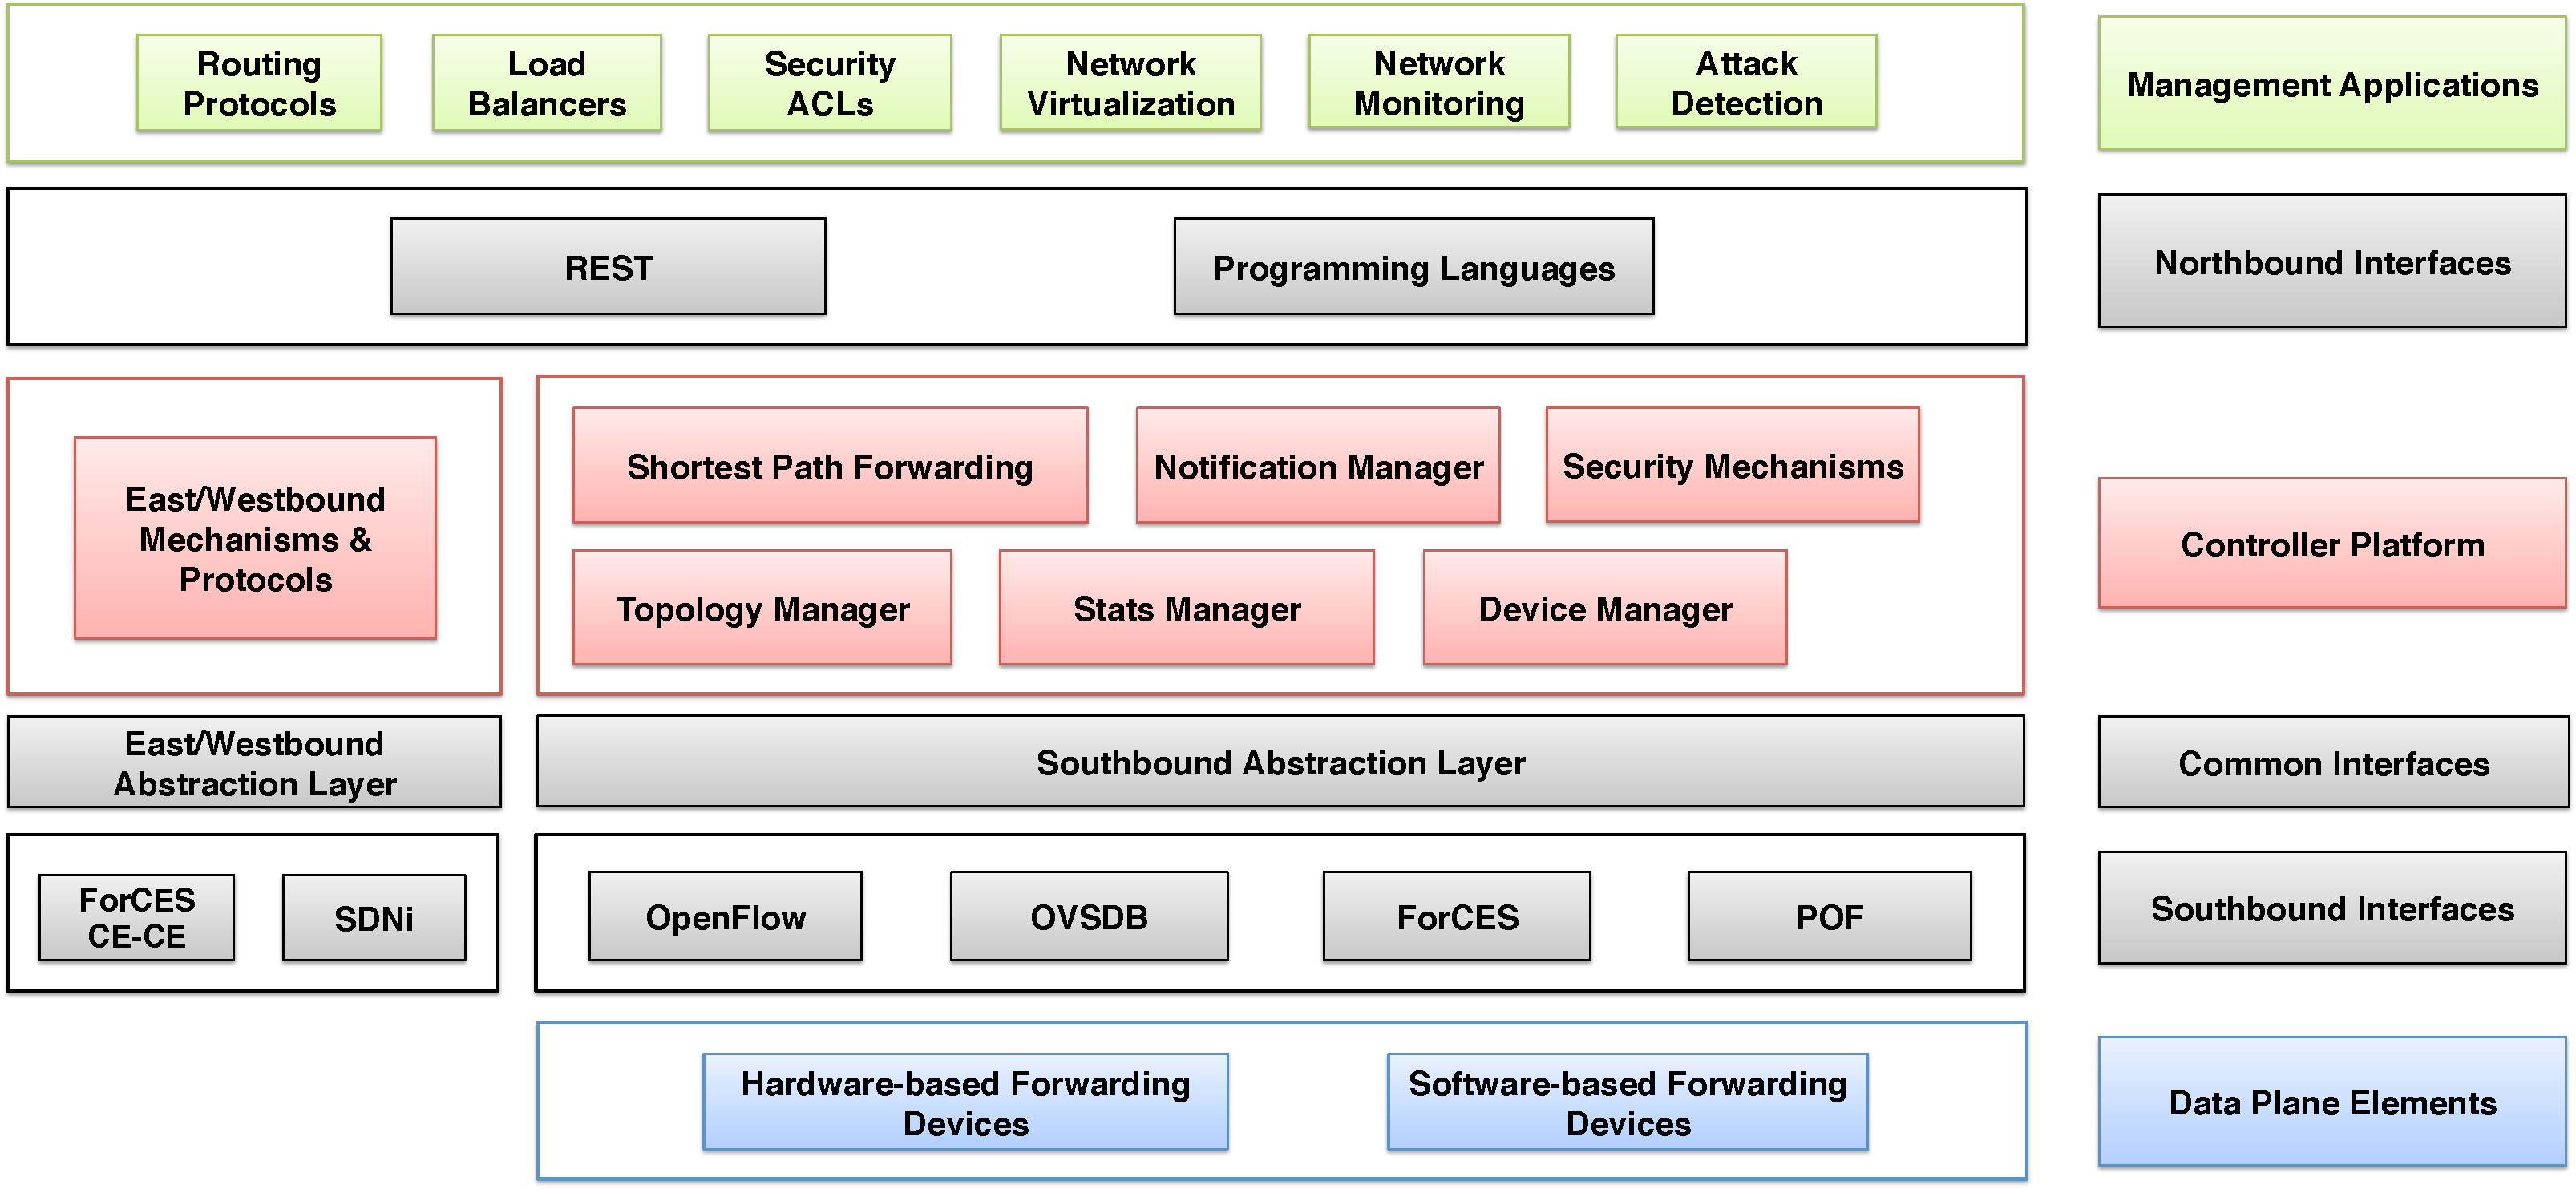
\includegraphics[width=0.85\textwidth]{figures/fig8_sdn_control_platform.pdf}
\caption{SDN control platforms: elements, services and interfaces}
\label{fig:controlplatformarch}
\end{figure*}

There are at least three relatively well-defined layers in most of the existing control platforms: 
(\textit{i}) the application, orchestration and services; (\textit{ii})  the core controller functions, and 
(iii) the elements for southbound communications. The connection at the upper-level layers is based on northbound interfaces such as REST APIs~\cite{richardson2008restful}  and programming languages such as FML~\cite{hinrichs2009}, Frenetic~\cite{foster2011} and NetCore~\cite{monsanto2012}. 
On the lower-level part of a control platform, southbound APIs and protocol plugins interface the forwarding elements. % and the controller platforms. 
The core of a controller platform can be characterized as a combination its base network service functions and the various interfaces. 


\vspace{2mm}
\noindent \textit{Core controller functions}

The base network service functions are what we consider the essential functionality all controllers should provide.
As an analogy, these functions are like base services of operating systems, 
such as program execution, I/O operations control, communications, protection, and so on. 
These services are used by other operating 
system level services and user applications. 
In a similar way, functions such as topology, statistics, notifications and device management, together with shortest path forwarding and security mechanisms are essential network control functionalities that network applications may use in building its logic.
For instance, the notification manager should be able to receive, process, and forward events (e.g., alarm notifications, security alarms, state changes)~\cite{onf2013-2}.
Security mechanisms are another example, as they are critical components to provide basic isolation and security enforcement between services and applications.
For instance, rules generated by high priority services should not be overwritten with rules created by applications with a lower priority.

%On the controller platform, network virtualization services are available for creating and managing 
%virtual tenant networks, traffic redirection services that can be used by routing and security services, 
%distributed overlay virtual Ethernet to deal with scenarios where overlays are required between segments 
%or sites of the network domain, among other specialized functions that may be needed by different services 
%and applications. The number and diversity of specialized services can significantly vary depending on the 
%target deployment scenario. While cloud infrastructure can require cloud integration and virtual tenant 
%network coordinators, these services may not be needed in a common enterprise network deployment.
%Another example could be deployment use cases requiring specialized IP multicasting services~\cite{kotani2012}.
%Therefore, while some services are of common use on most of the SDN deployment and can be considered as 
%essential services of a network operating systems, others are added on-demand accordingly the requirements 
%of the respective target environments.


\vspace{2mm}
\noindent \textit{Southbound}

On the lower-level of control platforms, the southbound APIs can be seen as a layer of device drivers.
They provide a common interface for the upper layers, while allowing a control platform to use different 
southbound APIs (e.g., OpenFlow, OVSDB, ForCES) and protocol plugins to manage existing or new physical or 
virtual devices (e.g., SNMP, BGP, NetConf). This is essential both for backward compatibility and heterogeneity, 
i.e., to allow multiple protocols and device management connectors. Therefore, on the data plane, a mix of physical devices, virtual devices (e.g., Open vSwitch~\cite{listofcontributors2013,pfaff2009}, vRouter~\cite{singla2013}) and a variety of device interfaces (e.g., OpenFlow, OVSDB, of-config~\cite{onf2013-1}, NetConf, and SNMP) can co-exist.

Most controllers support only OpenFlow as a southbound API. Still, a few of them, such as OpenDaylight, 
Onix and HP VAN SDN Controller, offer a wider range of southbound APIs and/or protocol plugins. Onix 
supports both the OpenFlow and OVSDB protocols. The HP VAN SDN Controller has other southbound connectors 
such as L2 and L3 agents. OpenDaylight goes a step beyond by providing a Service Layer Abstraction (SLA) 
that allows several southbound APIs and protocols to co-exist in the control platform. For instance, its 
original architecture was designed to support at least seven different protocols and plugins: OpenFlow, OVSDB~\cite{pfaff2013-1}, NETCONF~\cite{enns2011-1}, PCEP~\cite{vasseur2009}, SNMP~\cite{harrington2002}, BGP~\cite{rekhter2006} and LISP Flow Mapping~\cite{opendaylight2013}. Hence, OpenDaylight is one of 
the few control platforms being conceived to support a broader integration of technologies in a single 
control platform.


\vspace{2mm}
\noindent \textit{Eastbound and Westbound}

East/westbound APIs, as illustrated in Figure~\ref{fig:eastwestbounds}, are a special case of interfaces 
required by distributed controllers.
Currently, each controller implements its own east/westbound API. The functions of these interfaces include
import/export data between controllers, algorithms for data consistency models, and monitoring/notification 
capabilities (e.g., check if a controller is up or notify a take over on a set of forwarding devices).

\begin{figure}[ht]
\centering
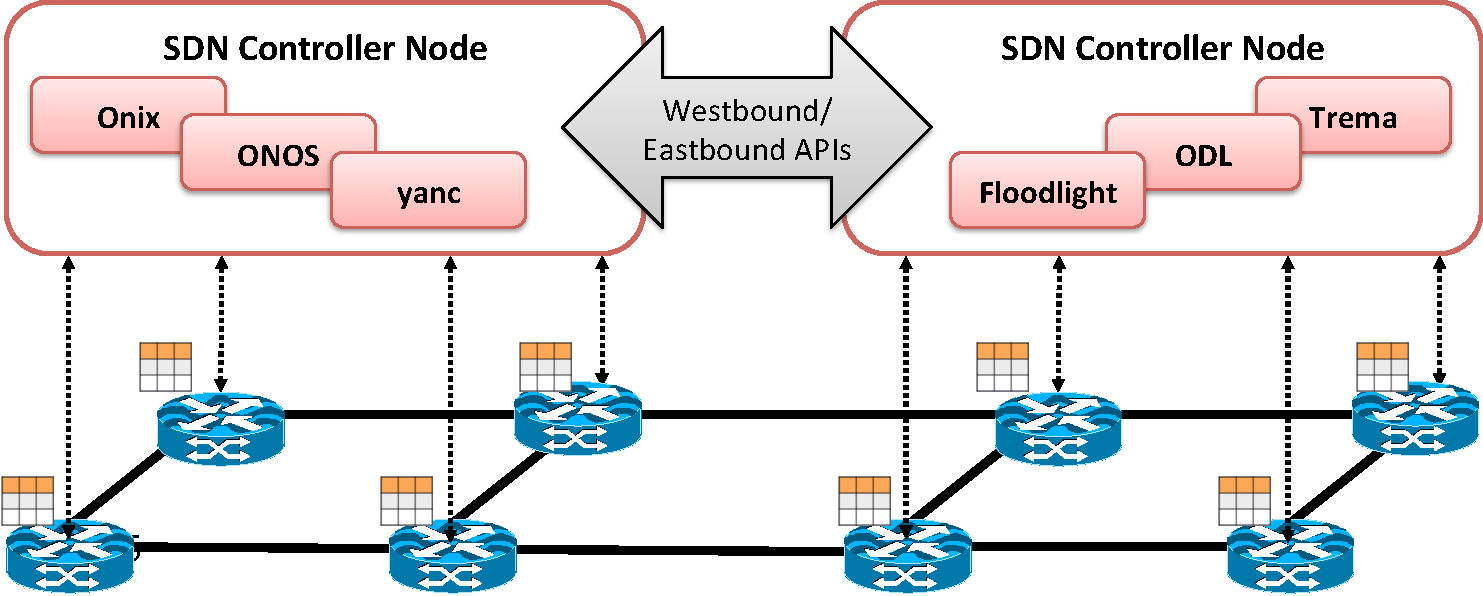
\includegraphics[width=0.99\columnwidth]{figures/fig7_sdn_eastwestbound.pdf}
\caption{Distributed controllers: east/westbound APIs.}
\label{fig:eastwestbounds}
\end{figure}

Similarly to southbound and northbound interfaces, east/westbound APIs are essential components of 
distributed controllers. 
To identify and provide common compatibility and interoperability between 
different controllers, it is necessary to have standard east/westbound interfaces. 
%Examples of early 
%initiatives that propose standard communication protocols and/or mechanisms between distinct control 
%nodes are SDNi~\cite{yin2012}, ForCES CE-CE interface~\cite{doria2010,wang2011-1}, 
%and ForCES Intra-NE mechanisms~\cite{ogawa2013}. 
For instance, SDNi~\cite{yin2012} defines 
common requirements to coordinate flow setup and exchange reachability information across multiple 
domains. 
In essence, such protocols can be used in an orchestrated and interoperable 
way to create more scalable and dependable distributed control platforms. Interoperability can be 
leveraged to increase the diversity of the control platform element. Indeed, diversity increases the 
system robustness by reducing the probability of common faults, such as software faults~\cite{garcia2013}.

%East/westbound APIs are essential building blocks for distributed or clustered controllers.
Other proposals that try to define interfaces between controllers include Onix data import/export functions~\cite{koponen-1}, ForCES CE-CE interface~\cite{doria2010,wang2011-1}, 
ForCES Intra-NE cold-standby mechanisms for high availability~\cite{ogawa2013}, and distributed data stores~\cite{botelho2013}. 
An east/westbound API requires advanced data distribution mechanisms such as the Advanced Message Queuing Protocol  (AMQP)~\cite{vinoski2006} used by
DISCO~\cite{phemius2013}, transactional databases and DHTs~\cite{ghodsi2006} ( as used in Onix~\cite{koponen-1}), or advanced algorithms for strong consistency and fault 
tolerance~\cite{botelho2013}.

In a multi-domain setup, east/westbound APIs may require also more specific communication protocols 
between SDN domain controllers~\cite{stallings2013}. Some of the essential functions of such 
protocols are to \textit{coordinate flow setup} originated by applications, \textit{exchange reachability 
information} to facilitate inter-SDN routing, \textit{reachability update} to keep the network state 
consistent, among others.

\vspace{2mm}
\noindent \textit{Northbound}

%%%NBI
%One of the important components of a network operating systems is the northbound interface.
Current controllers offer a quite broad variety of northbound APIs, such as ad-hoc APIs, RESTful APIs~\cite{richardson2008restful}, 
multi-level programming interfaces, file systems, among other more specialized APIs such as NVP NBAPI~\cite{koponen-1,koponen} and SDMN API~\cite{pentikousis2013}. %\cite{farooq2014}
 Section~\ref{sec:layer-north} is devoted to a more detailed discussion on the evolving layer of northbound APIs.  
 A second kind of northbound interfaces are those stemming out of SDN programming languages such as  
Frenetic~\cite{foster2011}, Nettle~\cite{voellmy2011-1},
NetCore~\cite{monsanto2012}, Procera~\cite{voellmy2012}, 
and Pyretic~\cite{monsanto2013}.  Section~\ref{sec:programminglanguages} gives a more detailed 
overview of the several existing programming languages for SDN.

%Programming languages are powerful northbound interfaces because they provide higher-level abstractions 
%to application developers, i.e., a programmer does not need to deal with low-level messages and events 
%from southbound interfaces (e.g., OpenFlow) that essentially emulate the behavior of a forwarding device.
%Programming languages such as Pyretic offer high-level policy description languages and logical predicates 
%to compose modular and reusable applications. More interestingly, some programming languages provide back-end 
%interfaces to simplify their integration with different network operating systems. For instance, Pyretic 
%requires only standard sockets and a simple OpenFlow client to be ported to different controllers~\cite{reich2013}.


{\renewcommand{\arraystretch}{1.4}
\begin{table*}[!htp]
\caption{Controllers classification}
\label{tab:controllers}
\begin{center}
\footnotesize
%\rowcolors{1}{lightgray}{white}
\begin{tabularx}{\linewidth}{p{2.94cm}Xp{2.29cm}p{1.47cm}p{0.75cm}p{1.35cm}p{2.1cm}p{0.9cm}}
\hline
\textbf{Name} & \textbf{Architecture} & \textbf{Northbound API} & \textbf{Consistency} & \textbf{Faults} & \textbf{License} & \textbf{Prog. language} & \textbf{Version}\\\hline
Beacon~\cite{erickson2013}     & centralized multi-threaded  & ad-hoc API & no & no & GPLv2 & Java & v1.0 \\\hline
DISCO~\cite{phemius2013} & distributed & REST & --- & yes & --- & Java & v1.1\\\hline
Floodlight~\cite{openflowhub.org2012} & centralized multi-threaded  & RESTful API & no & no & Apache & Java & v1.1 \\\hline
HP VAN SDN~\cite{hp2013-1} & distributed & RESTful API & weak & yes & --- & Java & v1.0 \\\hline
HyperFlow~\cite{tootoonchian2010}  & distributed               & --- & weak & yes & --- & C++ & v1.0 \\\hline
Kandoo~\cite{yeganeh2012}     & hierarchically distributed & --- & no & no & --- & C, C++, Python & v1.0 \\\hline
Onix~\cite{koponen-1}       & distributed               & NVP NBAPI   & weak, strong & yes & commercial & Python, C & v1.0 \\\hline
Maestro~\cite{cai2011}    & centralized multi-threaded  & ad-hoc API & no & no & LGPLv2.1 & Java & v1.0 \\\hline
Meridian~\cite{banikazemi2013} & centralized multi-threaded & extensible API layer & no & no & --- & Java & v1.0\\\hline
MobileFlow~\cite{pentikousis2013} & --- & SDMN API & --- & --- & --- & --- & v1.2 \\\hline
MuL~\cite{Saikia:2013:MuL}        & centralized multi-threaded  & multi-level interface & no & no & GPLv2 & C & v1.0 \\\hline
NOX~\cite{gude2008}       & centralized               & ad-hoc API  & no & no & GPLv3 & C++ & v1.0 \\\hline
NOX-MT~\cite{tootoonchian2012}     & centralized multi-threaded  & ad-hoc API & no & no & GPLv3 & C++ & v1.0 \\\hline
NVP Controller~\cite{koponen} & distributed & --- & --- & --- & commercial & --- & --- \\\hline
OpenContrail~\cite{junipernetworks2013-1} & --- & REST API & no & no & Apache 2.0 & Python, C++, Java & v1.0\\\hline
OpenDaylight~\cite{opendaylight2013} & distributed & REST, RESTCONF & weak & no & EPL v1.0 & Java & v1.\{0,3\} \\\hline
ONOS~\cite{krishnaswamy2013} & distributed & RESTful API & weak, strong & yes & --- & Java & v1.0 \\\hline
POX~\cite{mccauley2012}       & centralized               & ad-hoc API  & no & no & GPLv3 & Python & v1.0 \\\hline
ProgrammableFlow \cite{shimonishi2010} & centralized & --- & --- & --- & --- & C & v1.3 \\\hline
Ryu NOS~\cite{nippontelegraphandtelephonecorporation2012} & centralized multi-threaded & ad-hoc API & no & no & Apache 2.0 & Python & v1.\{0,2,3\}\\\hline
SNAC~\cite{appenzeller2011} & centralized & ad-hoc API & no & no & GPL & C++ & v1.0 \\\hline
Trema~\cite{takamiya2012}      & centralized multi-threaded  & ad-hoc API & no & no & GPLv2 & C, Ruby & v1.0 \\\hline
\textit{Unified Controller}~\cite{racherla2014} & --- & REST API & --- & --- & commercial & --- & v1.0 \\\hline
\textit{yanc}~\cite{monaco2013} & distributed & file system & --- & --- & --- & --- & --- \\\hline
\end{tabularx}
\end{center}
\end{table*}
}

\vspace{2mm}
\noindent \textit{Wrapping up remarks and platforms comparison}

Table~\ref{tab:controllers} shows a summary of some of the existing controllers with their respective 
architectures and characteristics.
As can be observed, most controllers are centralized and multi-threaded.
Curiously, the northbound API is very diverse. In particular, five controllers (Onix, Floodlight, MuL, Meridian and SDN Unified Controller) pay a bit more attention to this interface, as a statement
of its importance. Consistency models and fault tolerance are only present in Onix, HyperFlow, HP VAN SDN, 
and ONOS. Lastly, when it comes to the OpenFlow standard as southbound API, only Ryu supports its three 
major versions (v1.0, v1.2 and v1.3).

%A northbound API is an interface between the resources provided by the controller and applications. 
%It can be a programming language, a framework, or a standard set of functions provided by a library that facilitates the developer's life. 
%These APIs can also provide interoperability between different controllers in the sense that one application can be installed and executed on diverse controllers without any modification.
%The east/westbound APIs are more specific building blocks required by clustered or replicated controllers, i.e., they %are essential services of distributed network operating systems.
%These APIs should implement essential functions for data distribution, consistency models, and integrity guarantees, for instance.

%Essential network services represent the crucial and ``always needed'' network functions such as topology manager, device manager, and shortest path routing.
%Therefore, these services should be provided as built-in functions of controllers.

%Yet, the common abstraction layers are design artifacts to enable different east/westbound APIs, southbound APIs and protocol plug-ins to co-exist. 
%Therefore, they can be seen as a higher level common programming abstraction that suppress the details of lower level APIs, protocols and adaptors needed to connect and manage heterogeneous devices and systems.
%Accordingly, they provide standard programming interfaces for upper level frameworks and services such as programming frameworks and applications (e.g., common read and write methods, flow programming abstractions). 
%Underneath this layer a set of drivers and/or plugins can co-exist for integrating different data plane technologies.
%They are known as southbound APIs or connectors, representing protocols and plugins needed to manage diverse technologies such as OpenFlow, OVSDB, NETCONF, BGP, and SNMP.

%Another interesting thing to observe is that SDN domains~\cite{stallings2013} can be used in the context 
%of one or multiple infrastructure domains. Benefits and reasons for using multiple SDN domains include scalability,
%privacy, and incremental deployment. The scaling capability of a single controller node is not infinite, meaning 
%that it can handle only a limited number of devices. Moreover, privacy policies can be required in a per domain basis.
%For instance, carrier-grade network infrastructures and service providers have diverse kinds of customers that need
%different privacy policies.

%Incremental deployment is also a major requirement for infrastructure providers since it is infeasible to change all the legacy systems at once.
%Specially in transport and large-scale networks, incremental deployments of new control platforms and forwarding devices is a must have property.
%Changing routers, fabric, chassis switches, among other devices, is costly and has to pay off for infrastructure and service providers.

%From the security and dependability perspective it is worth emphasizing that most of the existing controllers are essentially monolithic applications~\cite{monaco2013,monsanto2013,foster2011,cai2011,nippontelegraphandtelephonecorporation2012,openflowhub.org2012,voellmy2011-1}, i.e., there is a domain specific programming language and/or a single resulting executable.
%Consequently, bugs in any part of the control platform (controller, application, module, etc.) can lead to severe consequences on the entire system.
%Even distributed controllers such as HyperFlow, Kandoo, and Onix are comprised of a set of monolithic distributed nodes.

%It is also worth mentioning that there are other research initiatives on controllers and control platforms such as clusters of controllers~\cite{yazici2012}, Hybrid Control Plane~\cite{martinez2011} to integrate OpenFlow Ethernet networks with GMPLS based networks, high performance controller for large multi-core architectures~\cite{theyalehaskellgroup2013}, and Distributed Controllers~\cite{macapuna2010} for data center networking.
%The Hybrid Control Plane~\cite{martinez2011} proposes distributed NOX-based controllers that work together through extended GMPLS protocols.
%The main idea is to provide an unified control platform between packet and circuit networks.
%In more specific use cases, distributed autonomous controllers are employed to manage data centers~\cite{macapuna2010}, for instance.
%In this case, the controllers allotting is done in a top of rack (TOR) basis for higher throughput (in a single TOR) and higher availability.

%Other initiatives propose algorithms for building clusters of controllers~\cite{yazici2012}.
%On the core of such solutions is a sort of coordination framework which helps on building and deploying clusters of controllers for environments requiring higher levels of scalability and reliability such as cloud scale data centers.
%Beacon, NOX, and Maestro were already used to prototype and evaluate coordination frameworks~\cite{yazici2012}.
%Experimental results show that a Beacon cluster is capable of achieving a throughput of six million flows per seconds in a modest set of four dual-core machines with low memory footprint and unmanaged gigabit connection.
%Although the throughput is lower that the one reported in ~\cite{erickson2013-1}, in which the experiments took advantage of a cluster with eight extra large computing nodes from Amazon's Elastic Computer Cloud (16 cores, more than 60GB of RAM, and 10Gb network), it increases approximately linearly with the number of nodes in the cluster.

To conclude, it is important to emphasize that the control platform is one of the critical points for 
the success of SDN~\cite{casemore2012-1}.
One of the main issues that needs to be address in this respect is interoperability. 
This is rather interesting, as it was the very first problem that southbound APIs (such as OpenFlow) tried to solve.
For instance, while WiFi and LTE networks~\cite{Kwan2010survey} need specialized control platforms such as MobileFlow~\cite{pentikousis2013} or SoftRAN~\cite{gudipati2013}, 
data center networks have different requirements that can be met with platforms such as Onix~\cite{koponen-1} or OpenDaylight~\cite{opendaylight2013}. 
For this reason, in environments where diversity of networking infrastructures is a reality, coordination and cooperation between different controllers is crucial. 
Standardized APIs for multi-controller and multi-domain deployments are therefore seen as an important step to achieve this goal.

\subsection{Layer V: Northbound Interfaces}
\label{sec:layer-north}

The North- and Southbound interfaces are two key abstractions of the SDN ecosystem. 
The southbound interface has already a widely accepted proposal (OpenFlow), but a common northbound 
interface is still an open issue.
At this moment it may still be a bit too early to define a standard northbound interface, as use-cases are still being worked out~\cite{dix2013}.
Anyway, it is to be expected a common (or a \emph{de facto}) northbound interface to arise as SDN evolves.
An abstraction that would allow network applications not to depend on specific implementations is important to explore the full potential of SDN 

The northbound interface is mostly a software ecosystem, not a hardware one as is the case of the southbound APIs.
In these ecosystems, the implementation is commonly the forefront driver, while standards emerge later and 
are essentially driven by wide adoption~\cite{guis2012}. Nevertheless, an initial and 
minimal standard for northbound interfaces can still play an important role for the future of SDN. 
Discussions about this issue have already begun ~\cite{dix2013,guis2012,salisbury2012-1,ferro2012,casemore2012,pepelnjak2012,johnson2012,little2013-1}, and a common consensus is that northbound APIs are indeed important but that it is indeed too early to define a single standard right now.
The experience from the development of different controllers will certainly be the basis for coming up with a common application level interface.

Open and standard northbound interfaces are crucial to promote application portability and interoperability among the different the control platforms.
A northbound API can be compared to the POSIX standard in operating systems, representing an abstraction that guarantees programming language and controller independence.
NOSIX~\cite{wundsam2012} is one of the first examples of an effort in this direction. It tries to 
define portable low-level (e.g., flow model) application interfaces, making southbound APIs such as OpenFlow 
look like ``device drivers''. However, NOSIX is not exactly a general purpose northbound interface, but 
rather a higher-level abstraction for southbound interfaces. Indeed, it could be part of the common 
abstraction layer in a control platform as the one described in Section~\ref{sec:controllers}.

Existing controllers such as Floodlight, Trema, NOX, Onix, and OpenDaylight propose and define their own northbound 
APIs~\cite{salisbury2012-1,chua2012}.
However, each of them has its own specific definitions.
Programming languages such as Frenetic~\cite{foster2011}, Nettle~\cite{voellmy2011-1}, NetCore~\cite{monsanto2012}, Procera~\cite{voellmy2012} and Pyretic~\cite{reich2013} also abstract the inner details of the controller functions and data plane behavior from the application developers.
Moreover, as we explain in 
Section~\ref{sec:programminglanguages}, programming languages can provide a wide range of powerful 
abstractions and mechanisms such as application composition, transparent data plane fault tolerance, 
and a variety of basic building blocks to ease software module and application development.

SFNet~\cite{yap2010} is another example of a northbound interface. It is a high-level API that 
translates application requirements into lower level service requests. However, SFNet has a limited scope, 
targeting queries to request the congestion state of the network and services such as bandwidth reservation 
and multicast.

Other proposals use different approaches to allow applications to 
interact with controllers. The \textit{yanc} control platform~\cite{monaco2013} explores 
this idea by proposing a general control platform based on Linux and abstractions such as the virtual file 
system (VFS). This approach simplifies the development of SDN applications as programmers are able to use
a traditional concept (files) to communicate with lower level devices and sub-systems.
 
Eventually, it is unlikely that a single northbound interface emerges as the winner, as the requirements for 
different network applications are quite different. APIs for security applications are likely to be different 
from those for routing or financial applications. One possible path of evolution for northbound APIs are 
vertically-oriented proposals, before any type of standardization occurs, a challenge the ONF has started 
to undertake in addition to open-source SDN controller platform developments (e.g., OpenDaylight, Floodlight,
OpenStack). 
%When and if this happens, the NBAPI might become more like an OS API (e.g., POSIX, iOS, Android), 
%to accommodate the potential wide range of applications that want a piece of the network.

\subsection{Layer VI: Language-based Virtualization}
\label{sec:virtualizationslicing}

Two essential characteristics of virtualization solutions are the capability of expressing modularity 
and of allowing different levels of abstractions while still guaranteeing desired properties such as protection.
For instance, virtualization techniques can allow different views of a single physical infrastructure.
As an example, one virtual ``big switch'' could represent a combination of several underlying forwarding devices.
This intrinsically simplifies the task of application developers as they do not need to think about the sequence of switches where forwarding rules have to be installed, but rather see the network as a 
simple ``big switch''.
Such kind of abstraction significantly simplify the development 
and deployment of complex network applications, such as advanced security related services.

Pyretic~\cite{reich2013} is an interesting example of a programming language that offers this type of high-level abstraction of network topology.
It incorporates this concept of abstraction by introducing network objects.
These objects consist of an abstract network topology and the sets of policies applied to it.
Network objects simultaneously hide information and offer the required services.

%An abstract topology can be a single big switch or a set of virtual switches spanned over the physical network.
%This means that Pyretic supports both ``one-to-many'' and ``many-to-one'' mappings, which empowers network 
%programmers with high flexible network topology abstractions for creating modular and composable SDN applications.
%For instance, a typical MAC-learning application is not suitable to learn the location of hosts in large networks.
%However, with topology abstractions, one can deploy the MAC-learning functionality only at the edge of the 
%network, where it is really needed and effective. 
%Beyond that, combine this application with a second one, 
%e.g., shortest-path routing and multicast trees, used to control the core of the network.

Another form of language-based virtualization is static slicing. 
This a scheme where the network is sliced by a compiler, based on application layer definitions.
The output of the compiler is a monolithic control program that has already slicing definitions and configuration commands for the network.
In such a case, there is no need for a hypervisor to dynamically manage the network slices.
Static slicing can be valuable for deployments with specific requirements, in particular those where higher performance and simple isolation guarantees are preferrable to
dynamic slicing.

One example of static slicing approach it the Splendid isolation~\cite{gutz2012}.
In this solution the network slices are made of 3 components:
(a) \textit{topology}, consisting of switches, ports, and links;
(b) \textit{mapping} of slice-level switches, ports and links on the network infrastructure;
(c) \textit{predicates on packets}, where each port of the slice's edge switches has an associated predicate.
The topology is a simple graph of the sliced nodes, ports and links.
Mapping will translate the abstract topology elements into the corresponding physical ones.
The predicates are used to indicate whether a packet is permitted or not to enter a specific slice. 
Different applications can be associated to each slice.
The compiler takes the combination of slices (topology, mapping, and predicates) and respective programs to generate a global configuration for the entire network. 
It also ensures that properties such as isolation are enforced among slices, i.e., no packets of a slice A can traverse to a slice B unless 
explicitly allowed.

Other solutions, such as libNetVirt~\cite{turull2012}, try to integrate heterogeneous technologies for creating 
static network slices. libNetVirt is a library designed to provide a flexible way to create and manage virtual 
networks in different computing environments. Its main idea is similar to the OpenStack Quantum 
project~\cite{quantumcommunicty2012}. While Quantum is designed for OpenStack (cloud environments), 
libNetVirt is a more general purpose library which can be used in different environments. Additionally, 
it goes one step beyond OpenStack Quantum by enabling QoS capabilities in virtual networks~\cite{turull2012}.
The libNetVirt library has two layers: (1) a generic network interface; and (2) technology specific device drivers 
(e.g., VPN, MPLS, OpenFlow). On top of the layers are the management applications and virtual network descriptions.
The OpenFlow driver uses a NOX controller to manage the underlying infrastructure, using OpenFlow rule-based flow 
tables to create isolated virtual networks. By supporting different technologies, it can be used as a bridging 
component in heterogeneous networks.

Table~\ref{tab:virtualizationsolutions} summarizes the hypervisor and non-hypervisor based virtualization 
technologies. 
As can be observed, only libNetVirt supports heterogeneous technologies, not restricting its 
application to OpenFlow-enabled networks. FlowVisor, AutoSlice and OpenVirteX allow multiple controllers, 
one per network slice. FlowN provides a container-based approach where multiple applications from different 
users can co-exist on a single controller. FlowVisor allows QoS provisioning guarantees by using VLAN PCP bits for priority queues.
SDN VE and NVP also provide their own provisioning methods for guaranteeing QoS.

{\renewcommand{\arraystretch}{1.4}
\begin{table*}[!htp]
\caption{Virtualization solutions}
\label{tab:virtualizationsolutions}
\begin{center}
\footnotesize
%\rowcolors{1}{lightgray}{white}
\begin{tabularx}{\textwidth}{p{3cm}p{3.1cm}p{3.1cm}p{2.6cm}X}
\hline
\textbf{Solution} & \textbf{Multiple controllers} & \textbf{Slicing} & \textbf{QoS ``guarantees''} & \textbf{Multi-technology} \\\hline
AutoSlice~\cite{bozakov2012} & yes, one per slice & VLAN tags & no & no, OF only\\\hline
FlowVisor~\cite{sherwood2009,azodolmolky2012} & yes, one per slice & virtual flow tables per slice &  yes (VLAN PCP bits) & no, OF only \\\hline
FlowN~\cite{drutskoy2012,drutskoy2013} & no (contained applications) & VLAN tags  & \textit{unknown} & no, OF only \\\hline
IBM SDN VE~\cite{racherla2014} & yes, a cluster of controllers & logical datapaths & yes (priority-based) & yes (VXLAN, OVS, OpenFlow) \\\hline
libNetVirt~\cite{turull2012} & no, one single controller & VLAN tags & no  & yes (e.g., VPN, MPLS, OpenFlow)\\\hline
NVP's Hypervisor~\cite{koponen} & yes, a cluster of controller & logical datapaths & yes & no, OVS only \\\hline
OpenVirteX~\cite{al-shabibi2014} & yes, one per slice & virtual flow tables per slice & \textit{unknown}  & no, OF only \\\hline 
Pyretic~\cite{reich2013} & no, one single controller & compiler time OF rules & no & no, OF only \\\hline
Splendid Isolation~\cite{gutz2012} & no, one single controller & compiler time VLANs & no  & no, OF only \\
\hline
\end{tabularx}
\end{center}
\end{table*}
}


\subsection{Layer VII: Programming languages}
\label{sec:programminglanguages}

Programming languages have been proliferating for decades. Both academia and industry have evolved 
from low-level hardware-specific machine languages, such as assembly for x86 architectures, to high-level 
and powerful programming languages such as Java and Python. The advancements towards more portable and 
reusable code has driven a significant shift on the computer industry~\cite{guzdial2008,farooq2014}.

Similarly, programmability in networks is starting to move from low level machine languages such as OpenFlow (``assembly'') to high-level programming languages~\cite{foster2011,hinrichs2009,voellmy2011-1,monsanto2012,voellmy2012,monsanto2013,koponen}.
Assembly-like machine languages, such as OpenFlow~\cite{mckeown2008} and POF~\cite{song2013,song2013-1}, essentially mimic the behavior of forwarding devices, forcing developers to spend too much time on low-level details
rather than on the problem solve.
Raw OpenFlow programs have to deal with hardware behavior details such as overlapping rules, the priority ordering of rules, and data-plane inconsistencies that arise from in-flight packets whose flow rules are under installation~\cite{foster2011,monsanto2012,ferguson2012}.
The use of these low-level languages makes it difficult to reuse software, to create modular and extensive code, and leads to a more error-prone development process~\cite{monsanto2013,nelson2013,katta2012}.

Abstractions provided by high level programming languages can significantly help address many 
of the challenges of these lower-level instruction sets~\cite{foster2011,hinrichs2009,voellmy2011-1,monsanto2012,voellmy2012,monsanto2013}.
In SDNs, high-level programming languages can be designed and used to:
\begin{enumerate}
\item create higher level abstractions for simplifying the task of programming forwarding devices;
\item enable more productive and problem-focused environments for network software programmers, speeding up development and innovation;
\item promote software modularization and code reusability in the network control plane;
\item foster the development of network virtualization.
\end{enumerate}

Several challenges can be better addressed by programming languages in SDNs.
For instance, in pure OpenFlow-based SDNs, it is hard to ensure that multiple tasks of a single application 
(e.g., routing, monitoring, access control) do not interfere with each other.
For example, rules generated for one task should not override the functionality of another task~\cite{foster2011,ferguson2012}.
Another example is when multiple applications run on a single controller~\cite{monsanto2013,ferguson2012,porras2012,shin2013-1,son2013}.
Typically, each application generates rules based on its own needs and policies without further knowledge about the rules generated by other applications. As a consequence, conflicting rules can be generated and installed in forwarding devices, which can create problems for network operation.
Programming languages and runtime systems can help to solve these problems that would be otherwise hard to prevent.

Important software design techniques such as code modularity and reusability are very hard to achieve using low-level programming models~\cite{monsanto2013}.
Applications thus built are monolithic and consist of building blocks that can not be reused in other applications.
The end result is a very time consuming and error prone development process.

Another interesting feature that programming language abstractions provide is the capability of 
creating and writing programs for virtual network topologies~\cite{reich2013,gutz2012}.
This concept is similar to object-oriented programming, where objects abstract both data and specific functions 
for application developers, making it easier to focus on solving a particular problem without worrying about 
data structures and their management. For instance, in an SDN context, instead of generating and installing 
rules in each forwarding device, one can think of creating simplified virtual network topologies that represent 
the entire network, or a subset of it. For example, the application developer should be able to abstract the 
network as an atomic big switch, rather than a combination of several underlying physical devices.
The programming languages or runtime systems should be responsible for generating and installing the lower-level 
instructions required at each forwarding device to enforce the user policy across the network. With such kind of 
abstractions, developing a routing application becomes a straightforward process. Similarly, a single physical 
switch could be represented as a set of virtual switches, each of them belonging to a different virtual network.
These two examples of abstract network topologies would be much harder to implement with low-level 
instruction sets. In contrast, a programming language or runtime system can more easily provide abstractions 
for virtual network topologies, as has already been demonstrated by languages such as Pyretic~\cite{reich2013}.

\vspace{2mm}
\noindent \textit{High-level SDN programming languages}


Low-level instruction sets suffer from several problems.
To address some of these challenges, higher-level programming languages have been proposed, with 
diverse goals, such as:
\begin{itemize}
\item Avoiding low-level and device-specific configurations and dependencies spread across the network, as happens
in traditional network configuration approaches; 
\item Providing abstractions that allow different management tasks to be accomplished through easy to understand and maintain network policies;
\item Decoupling of multiple tasks (e.g., routing, access control, traffic engineering);
\item Implementing higher-level programming interfaces to avoid low-level instruction sets;
\item Solving forwarding rules problems, e.g., conflicting or incomplete rules that can prevent a switch event to be triggered, in an automated way;
\item Addressing different race condition issues which are inherent to distributed systems;
\item Enhancing conflict-resolution techniques on environments with distributed decision makers;
\item Provide native fault-tolerance capabilities on data plane path setup;
\item Reducing the latency in the processing of new flows;
\item Easing the creation of stateful applications (e.g., stateful firewall).
\end{itemize}

Programming languages can also provide specialized abstractions to cope with other management requirements, 
such as monitoring~\cite{voellmy2012,foster2011,tootoonchian2010-1}.
For instance, the runtime system of a programming language can do all the ``laundry work'' of installing rules, polling 
the counters, receiving the responses, combining the results as needed, and composing monitoring queries in 
conjunction with other policies. Consequently, application developers can take advantage of the simplicity and 
power of higher level query instructions to easily implement monitoring modules or applications.

Another aspect of paramount importance is the portability of the programming language, necessary so that developers do not 
need to re-implement applications for different control platforms.
The portability of a programming language can be considered as a significant added value to the control plane ecosystem. 
Mechanisms such as decoupled back-ends could be key architectural ingredients to enable platform portability.
Similarly to the Java virtual machine, a portable northbound interface will easily allow applications to run on different controllers without requiring any modification.
As an example, the Pyretic language requires only a standard socket interface and a simple OpenFlow client on the target controller 
platform~\cite{monsanto2013}.

Several programming languages have been proposed for SDNs, as summarized in Table~\ref{tab:programminglanguages}.
The great majority propose abstractions for OpenFlow-enabled networks.
The predominant programming paradigm is the declarative one, with a single exception, Pyretic, which is an imperative language. 
Most declarative languages are functional, while but there are instances of the logic and reactive types.
The purpose -- i.e., the specific problems they intend to solve -- and the expressiveness power vary from language to 
language, while the end goal is almost always the same: to provide higher-level abstractions to facilitate the 
development of network control logic.

{\renewcommand{\arraystretch}{1.4}
\begin{table*}[!htp]
\caption{Programming languages}
\label{tab:programminglanguages}
\begin{center}
\footnotesize
%\rowcolors{1}{lightgray}{white}
\begin{tabularx}{\linewidth}{p{2cm}p{4cm}X}
\hline
\textbf{Name} & \textbf{Programming paradigm} & \textbf{Short description/purpose} \\\hline
FatTire~\cite{reitblatt2013}  & declarative (functional) & Uses regular expressions to allow programmers to describe network paths and respective fault-tolerance requirements. \\\hline
Flog~\cite{katta2012}  & declarative (logic), event-driven & Combines ideas of FML and Frenetic, providing an event-driven and forward-chaining logic programming language. \\\hline
FlowLog~\cite{nelson2013} & declarative (functional) & Provides a finite-state language to allow different analysis, such as model-checking.\\\hline
FML~\cite{hinrichs2009} & declarative (dataflow, reactive) & High level policy description language (e.g., access control).  \\\hline
Frenetic~\cite{foster2011} & declarative (functional) & Language designed to avoid race conditions through well defined high level programming abstractions.  \\\hline
HFT~\cite{ferguson2012}  & declarative (logic, functional) & Enables hierarchical policies description with conflict-resolution operators, well suited for decentralized decision makers. \\\hline
Maple~\cite{voellmy2013} & declarative (functional) & Provides a highly-efficient multi-core scheduler that can scale efficiently to controllers with 40+ cores. \\\hline
Merlin~\cite{soule2013} & declarative (logic) & Provides mechanisms for delegating management of sub-policies to tenants without violating global constraints. \\\hline
nlog~\cite{koponen} & declarative (functional) &  Provides mechanisms for data log queries over a number of tables. Produces immutable tuples for reliable detection and propagation of updates. \\\hline
Nettle~\cite{voellmy2011-1}   & declarative (functional, reactive) & Based on functional reactive programming  principles in order to allow programmers to deal with streams instead of events.   \\\hline
NetCore~\cite{monsanto2012}  & declarative (functional) & High level programming language that provides means for expressing packet-forwarding policies in a high level.  \\\hline
Procera~\cite{voellmy2012}  & declarative (functional, reactive) & Incorporates a set of high level abstractions to make it easier to describe reactive and temporal behaviors.  \\\hline
Pyretic~\cite{monsanto2013}  & imperative & Specifies network policies at a high level of abstraction, offering transparent composition and topology mapping. \\\hline
\end{tabularx}
\end{center}
\end{table*}
}


% FIXME: think about it... this last part can be eventually suppressed
Programming languages such as FML~\cite{hinrichs2009}, 
Nettle~\cite{voellmy2011-1}, and Procera~\cite{voellmy2012}
are functional and reactive.
Policies and applications written in these languages are based on reactive actions triggered by events (e.g., a new host connected to the network, or the current network load).
Such languages allow users to declaratively express different network configuration rules such as access control lists (ACLs), virtual LANs (VLANs), and many others.
Rules are essentially expressed as allow-or-deny policies, which 
are applied to the forwarding elements to ensure the desired network behavior.

Other SDN programming languages such as Frenetic~\cite{foster2011},
Hierarchical Flow Tables (HFT)~\cite{ferguson2012}, NetCore~\cite{monsanto2012}, and
Pyretic~\cite{monsanto2013}, were designed with the simultaneous goal of efficiently expressing packet-forwarding policies and dealing with overlapping rules of different applications, offering advanced operators for parallel and sequential composition of software modules.
To avoid overlapping conflicts, Frenetic disambiguates rules 
with overlapping patterns by assigning different integer priorities, while HFT uses hierarchical policies with 
enhanced conflict-resolution operators.

\textit{See-every-packet} abstractions and race-free semantics also represent interesting features provided 
by programming languages (such as Frenetic~\cite{foster2011}). 
The former ensures that \emph{all} control packets will be available for analysis, sooner or later, while the latter provides the mechanisms for
suppressing unimportant packets. As an example, packets that arise from a network race condition, such as due to a concurrent flow 
rule installation on switches, can be simply discarded by the runtime system.

Advanced operators for parallel and sequential composition help bind (through internal workflow operators) 
the key characteristics of programming languages such as Pyretic~\cite{monsanto2013}. Parallel 
composition makes it possible to operate multiple policies on the same set of packets, while sequential 
composition facilitates the definition of a sequential workflow of policies to be processed on a set of 
packets. Sequential policy processing allows multiple modules (e.g., access control and 
routing) to operate in a cooperative way.
By using sequential composition complex applications can be built out of a combination of different modules (in a similar way as pipes can be used to build sophisticated Unix applications).

Further advanced features are provided by other SDN programming languages.
FatTire~\cite{reitblatt2013} is an example of a declarative language that heavily relies on regular 
expressions to allow programmers to describe network paths with fault-tolerance requirements. For instance, 
each flow can have its own alternative paths for dealing with failure of the primary paths. 
Interestingly, this feature is provided in a very programmer-friendly way, with the application programmer having only to use regular 
expressions with special characters, such as an asterisk. In the particular case of FatTire, an asterisk will produce the same behavior 
as a traditional regular expression, but translated into alternative traversing paths.
%As an example, imagine 
%that a particular flow has to pass through a deep packet inspection middlebox. If in case it can use any path 
%from the ingress switch to the DPI device, a regular expression can be used to declare that the flow is allowed 
%to pass any path (*) leading to the DPI system. Consequently, if the primary path fails, alternative paths will 
%be available and ready to thwart the problem.

Programming languages such as FlowLog~\cite{nelson2013} and Flog~\cite{katta2012} bring 
different features, such as model checking, dynamic verification and stateful middleboxes. For instance, using a programming language such as Flog, it is possible to build a 
stateful firewall application with only five lines of code~\cite{katta2012}.

Merlin~\cite{soule2013} is one of the first examples of unified framework for controlling different network components, such as forwarding devices, middleboxes, and end-hosts.
An important advantage is backward-compatibility with existing systems.
To achieve this goal, Merlin generates specific code for each type of component.
Taking a policy definition as input, Merlin's compiler determines forwarding 
paths, transformation placement, and bandwidth allocation.
The compiled outputs are sets of component-specific 
low-level instructions to be installed in the devices.
Merlin's policy language also allows operators to delegate the control of a sub-network to tenants, while ensuring isolation.
This delegated control is expressed by means of policies that can be further refined 
by each tenant owner, allowing them to customize policies for their particular needs. 
%The verification capability 
%is a natural requirement to avoid that different tenants specialize policies in such a way that it can cause 
%interference on other tenants. To avoid problems among tenants, the verification process has to guarantee 
%isolation, i.e., check whether the extended policy of a tenant is a valid specialization of the original 
%policy and does not violate any isolation requirement. Finally, the framework tries also to distribute 
%enforcement mechanisms (e.g., bandwidth constraints) to end-hosts, reducing the contention in forwarding 
%elements.

Other recent initiatives (e.g., systems programming languages~\cite{casey2013}) 
target problems such as detecting anomalies to improve the security of network protocols (e.g., OpenFlow), 
and optimizing horizontal scalability for achieving high throughput in applications running on multicore 
architectures~\cite{voellmy2013}.
%One of the key ideas behind systems programming languages 
%is to offer support new ways of expressing network protocol message structures and constraints. With a smart 
%enough compiler, these definitions can be used to identity and take countermeasures against known protocol 
%vulnerabilities, for instance.

%One arguable dichotomy of SDN is its reliance on software artefacts expected to yield a high-level defined, 
%flexible yet robust networking paradigm (cf.~\cite{doyle2005}).
Most of the value of SDN will come from the network managements applications built on top of the infrastructure.
Advances in high-level programming languages are a fundamental component to the success of a prolific SDN 
application development ecosystem. To this end, efforts are undergoing to shape forthcoming standard 
interfaces (cf.~\cite{kuzniar2013}) and towards the realization of integrated development 
environments (e.g., NetIDE~\cite{facca2013}) with the goal of fostering the development of a myriad of SDN applications.
We discuss these next.

\subsection{Layer VIII: Management applications}

Management applications can be seen as the ``network brains''. 
They implement the control-logic that will be translated into commands to be installed in the data plane, dictating the behavior of the forwarding devices.
Taking a simple application as routing as an example. 
The logic of this application is to define the path through which packets will flow from 
a point A to a point B.
To achieve this goal a routing application has to, based on the topology input, decide on the path to use and instruct the controller to install the 
respective forwarding rules in all forwarding devices on the chosen path, from A to B.

Software-defined networks can be deployed on any traditional network environment, from home and enterprise networks to data centers and Internet exchange points.
Such variety of environments has led to a wide array of management applications.
Existing network management applications perform traditional functionality such as routing, load balancing, and security policy enforcement, but also explore novel approaches, such as reducing power consumption . 
Other examples include fail-over and reliability functionalities to the data plane, end-to-end QoS enforcement, network virtualization, mobility management in wireless networks, among many others.

%Figure~\ref{fig:controllerplusapps} illustrates a controller with a set of three independent groups of applications.
%The first is a routing layer with two applications, discovery and intradomain routing.
%It receives LLD packets from switches and updates the routing table, which is used by the route flow module to configure paths for new flows.
%In the second group we have the security policy enforcement applications.
%For instance, a new user will have to authenticate as soon as he connects to the network, either wired or wireless.
%Depending on his authorizations, distinct security policies can be applied to flows belonging to the user.
%As a simple example we can consider the case of a visitor that will be isolated in a special network slice, which allows him to only have access to Internet services (e.g., HTTP and HTTPS).
%The third group is a routing and load balancing layer.
%For instance, some services may be directly accessed by any user, while others may require a load balancing policy.
%The second and third groups of applications generate an output consisting of flow rules for the underlying network infrastructure, which are carried out by the controller to the forwarding elements.
%A single flow setup may require the configuration of several switches across the network.
%
%\begin{figure}[ht]
%\centering
%\includegraphics[width=\columnwidth]{figures/sdn-controller-apps-v1.pdf}
%\caption{A controller and applications}
%\label{fig:controllerplusapps}
%\end{figure}

Despite the wide variety of use cases, most SDN applications can be grouped in one of five categories: traffic engineering, mobility and wireless, measurement and monitoring, security and dependability and data center networking.
Table~\ref{tab:managementapplications} summarizes several applications categorized as such, stating their main purpose, controller where it was implemented/evaluated, and southbound API used.

{\renewcommand{\arraystretch}{1.4}
\begin{table*}[!htp]
\caption{Management applications and services}
\label{tab:managementapplications}
\begin{center}
\footnotesize
%\rowcolors{1}{lightgray}{white}
\begin{tabularx}{\linewidth}{p{2cm}p{3.2cm}p{5.1cm}Xp{3.5cm}}
\hline
\textbf{Group} & \textbf{Solution/Application} & \textbf{Main purpose} & \textbf{Controller} & \textbf{Southbound API} \\
\hline
\multirow{12}{*}{\begin{minipage}{2cm}Traffic \\engineering\end{minipage}} 
& ALTO VPN~\cite{scharf2013} & on-demand VPNs & NMS~\cite{stiemerling2014ALTODeployment,alimi2013} & SNMP \\
& Aster*x~\cite{handigol2009}       & load balancing             &  NOX & OpenFlow      \\
& ElasticTree~\cite{heller2010}   & energy aware routing       &  NOX & OpenFlow      \\
& Hedera~\cite{al-fares2010}        & scheduling / optimization  &  --- & OpenFlow  \\
& In-packet Bloom filter~\cite{macapuna2010}        & load balancing  &  NOX & OpenFlow  \\
& OpenQoS~\cite{egilmez2012} & dynamic QoS routing for multimedia apps & Floodlight  & OpenFlow \\
& Plug-n-Serve~\cite{handigol2009-1}  & load balancing             &  NOX & OpenFlow      \\
& QNOX~\cite{jeong2012}          & QoS enforcement                &  NOX & Generalized OpenFlow \\
& QoS framework~\cite{kim2010} & QoS enforcement                &  NOX & OF with QoS extensions \\
& QoSFlow~\cite{ishimori2013} & multiple packet schedulers to improve QoS & --- & OpenFlow\\
& SIMPLE~\cite{qazi2013-1}  & middlebox-specific ``traffic steering'' & Extended POX & OpenFlow  \\
& ViAggre SDN~\cite{skoldstrom2013-1} & divide and spread forwarding tables & NOX & OpenFlow\\
\hline
\multirow{9}{*}{\begin{minipage}{2cm}Mobility \\\& \\Wireless\end{minipage}} 
& CROWD~\cite{ali-ahmad2013} & overlapping of LTE and WLAN cells & --- & OpenFlow \\
& CloudMAC~\cite{vestin2013} & outsourced processing of WLAN MACs & --- & OpenFlow \\
& FAMS~\cite{yamasaki2011} & flexible VLAN system based on OpenFlow & ProgrammableFlow & OpenFlow \\
& MobileFlow~\cite{pentikousis2013} & flow-based model for mobile networks & MobileFlow & SDMN API\\
& Odin~\cite{suresh2012} & smooth hand-off and load balancing & Floodlight & OpenFlow \\
& OpenRAN~\cite{yang2013} & vertical programmability and virtualization & --- & --- \\
& OpenRoads~\cite{yap2010-1} & control of the data path using OpenFlow & FlowVisor & OpenFlow \\
& SoftRAN~\cite{gudipati2013} & load balancing and interference management & --- & Femto API~\cite{smallcellforum2013,Chandrasekhar2008} \\
\hline
\multirow{7}{*}{\begin{minipage}{2cm}Measurement \\\& \\Monitoring\end{minipage}} 
& BISmark~\cite{kim2013} & active and passive measurements & Procera framework & OpenFlow \\
& FleXam~\cite{shirali-shahreza2013} & flexible sampling extension for OpenFlow & --- & --- \\
& FlowSense~\cite{yu2013} & measure link utilization in OF networks & --- & OpenFlow \\
& measurement model~\cite{jose2011} & model for OF switch measurement tasks & --- & OpenFlow \\
& OpenSketch\,\cite{yu2013-1} & separated measurement data plane & OpenSketch & ``OpenSketch sketches'' \\
& OpenTM~\cite{tootoonchian2010-1} & traffic matrix estimation tool & NOX & OpenFlow \\
& PaFloMon\,\cite{argyropoulos2012} & passive monitoring tools defined by users & FlowVisor & OpenFlow \\
\hline
\multirow{15}{*}{\begin{minipage}{2cm}Security \\\& \\Dependability\end{minipage}} 
& Active security~\cite{hand2013} & integrated security using network feedback control & Floodlight & OpenFlow \\
& AVANT-GUARD~\cite{shin2013-3} & DoS security specific extensions to OF & POX & OpenFlow \\
& CloudWatcher~\cite{shin2012}  & framework for monitoring clouds & NOX & OpenFlow      \\
& DDoS detection~\cite{braga2010-1}     & attacks detection and mitigation    &  NOX & OpenFlow      \\
& Elastic IP and Security Group~\cite{stabler2012}  & an SDN based implementation of Amazon's Elastic IP and Security Groups & NOX & OpenFlow   \\
& Ethane~\cite{casado2007-1}   & flow-rule enforcement (match/action)&  Ethane controller & first instance of OpenFlow  \\
& FortNOX ~\cite{porras2012}    & security flow rules prioritization &  NOX & OpenFlow      \\
& FRESCO ~\cite{shin2013-1}    & framework for security services composition & NOX & OpenFlow      \\
& LiveSec~\cite{wang2012-1}       & security policy enforcement          &  NOX & OpenFlow      \\
& NetFuse~\cite{wang2013} & protection against OF traffic overload & --- & OpenFlow \\
& OF-RHM~\cite{jafarian2012}    & random host mutation (defense) &  NOX & OpenFlow      \\
& OpenSAFE~\cite{ballard2010} & direct spanned net traffic in arbitrary ways & NOX & OpenFlow \\
& Reliable multicasting~\cite{kotani2012} & reduce packet loss when failures occur & Trema & OpenFlow \\
& SANE~\cite{casado2006}       & security policy enforcement         &  SANE controller & SANE header (pre-OpenFlow) \\
& VAVE~\cite{yao2011} & source address validation with a global view & NOX & OpenFlow \\
\hline
\multirow{7}{*}{\begin{minipage}{2cm}Data Center \\Networking\end{minipage}} 
& Big Data Apps ~\cite{wang2012} & optimize network utilization & --- & OpenFlow   \\
& CloudNaaS~\cite{benson2011} & networking primitives for cloud applications & NOX &  OpenFlow  \\
& FlowComb~\cite{das2013} & predicts application workloads & NOX & OpenFlow \\
& FlowDiff~\cite{arefin2013} & detects operational problems & FlowVisor & OpenFlow \\
& LIME~\cite{keller2012} & live network migration & Floodlight & OpenFlow      \\
& NetGraph ~\cite{raghavendra2012} & graph queries for network management & --- & OpenFlow, SNMP   \\
& OpenTCP~\cite{ghobadi2013} & dynamic and programmable TCP adaptation & --- & --- \\
\hline
\end{tabularx}
\end{center}
\end{table*}
}

\vspace{2mm}
\noindent \textit{Traffic engineering}

Several traffic engineering applications have been proposed, including 
ElasticTree~\cite{heller2010}, Hedera~\cite{al-fares2010},
OpenFlow-based server load balancing~\cite{wang2011},
Plug-n-Serve~\cite{handigol2009-1} and Aster*x~\cite{handigol2009},
In-packet Bloom filter~\cite{macapuna2010},
SIMPLE~\cite{qazi2013-1}, QNOX~\cite{jeong2012}, QoS framework~\cite{kim2010},
ALTO~\cite{scharf2013}, and ViAggre SDN~\cite{skoldstrom2013-1}.
The main goals of most applications is to engineer traffic with the aim of minimizing power consumption, maximizing aggregate network utilization, providing optimized load balancing, and other generic traffic optimization techniques.

Load balancing was one of the first applications envisioned for SDN/OpenFlow.
Different algorithms and techniques have been proposed for this purpose~\cite{wang2011,handigol2009,handigol2009-1}. 
One particular concern is the scalability of these solutions.
A technique to allow this type of applications to scale is to use wildcard-based rules to perform proactive load balancing~\cite{wang2011}.
Wildcards can be utilized for aggregating clients requests based on the ranges of IP prefixes, for instance, allowing the distribution and directing of large groups of client requests without requiring controller intervention for every new flow
In tandem, operation in reactive mode may still be used when traffic bursts are detected.
The controller application needs to monitor the network traffic and use some sort of 
threshold in the flow counters to redistribute clients among the servers when bottlenecks are likely to happen.

SDN load-balancing also simplifies the placement of network services in the network~\cite{handigol2009-1}.
Every time a new server is installed, the load-balancing service can take the appropriate actions to seamlessly distribute the traffic among the 
available servers, taking into consideration both the network load and the available computing capacity of the respective servers.
This simplifies network management and provides more flexibility to network operators.
% assumes that web services and computing resources are installed in the network in an arbitrary way, as it commonly happens in an university campus.
%It means that operators of these environments do not have a fine-grained control over the load distribution (e.g., placement of servers and current network traffic in all subnets) on the network when new resources need to be installed, for instance.
%Therefore, Aster*x is different from traditional load balancers in the sense that it uses a more global view of the network conditions to apply load balancing policies.
%As an example, we could have two servers A and B both of them with the same processing capacities.
%However, network traffic bottlenecks are more frequent between clients and the server B due to other services running on the same segment of the network.
%Consequently, the incoming traffic should not always be of 50\% for each server.
%Server A, despite having the exact same processing power, can receive more traffic load because its network path is less likely to have bottlenecks.

Existing southbound interfaces can be used for actively monitoring the data plane load.
This information can be leveraged to optimize the energy consumption of the network~\cite{heller2010}. 
By using specialized optimization algorithms and diversified configuration options, it is possible to meet the 
infrastructure goals of latency, performance, and fault tolerance, for instance, while reducing power consumption.
With the use of simple techniques, such as shutting down links and devices intelligently in response to traffic load dynamics, data center operators can save up to 50\% of the network energy in normal traffic 
conditions~\cite{heller2010}. 

One of the important goals of data center networks is to avoid or mitigate the effect of network bottlenecks on the operation of the computing services offered.
Linear bisection bandwidth is a technique that can be adopted for traffic patterns that stress the network by exploring path diversity in a data center 
topology.
Such technique has been proposed in an SDN setting, allowing the maximization of aggregated network utilization with minimal scheduling overhead~\cite{al-fares2010}. 

SDN can also be used to provide a fully automated system for controlling the configuration of routers.
This can be particularly useful in scenarios that apply virtual aggregation~\cite{ballani2009} .
This technique allows network operators to reduce the data replicated on routing tables, which 
is one of the causes of routing tables' growth~\cite{meyer2007}. 
A specialized routing application~\cite{skoldstrom2013-1} can calculate, divide and configure the routing tables of the different routing devices through a southbound API such 
as OpenFlow.

Traffic optimization is another interesting application for large scale service providers, where dynamic scale-out 
is required. For instance, the dynamic and scalable provisioning of VPNs in cloud infrastructures, using protocolols
such as ALTO~\cite{alimi2013}, can be simplified through an SDN-based approach~\cite{scharf2013}.

Other applications that perform routing and traffic engineering include application-aware 
networking for video streaming~\cite{jarschel2013} and improved QoS by employing multiple packet 
schedulers~\cite{ishimori2013} and other techniques~\cite{kim2010,jeong2012,egilmez2012, kumar2013}.

\vspace{2mm}
\noindent \textit{Mobility \& wireless}

The current distributed control plane of wireless networks is suboptimal for managing the limited 
spectrum, allocating radio resources, implementing handover mechanisms, managing interference, and performing efficient load-balancing between cells.
SDN-based approaches represent an opportunity for making it easier to deploy and manage different types of wireless networks, such as WLANs and cellular 
networks~\cite{suresh2012,yap2010-1,ali-ahmad2013,gudipati2013,li2012,jin2013}.
Traditionally hard-to-implement but desired features are indeed becoming a reality with the SDN-based wireless networks. 
These include seamless mobility through efficient hand-overs~\cite{suresh2012,dely2011,li2012}, load balancing~\cite{suresh2012,gudipati2013}, creation of on-demand virtual access points (VAPs)~\cite{suresh2012,vestin2013}, downlink scheduling (e.g., an OpenFlow switch can do a rate shaping or time division) ~\cite{vestin2013}, dynamic spectrum usage~\cite{vestin2013}, enhanced inter-cell 
interference coordination~\cite{vestin2013,li2012}, device to device offloading (i.e., decide in when and how LTE transmissions should be offloaded to users adopting the D2D paradigm~\cite{yang2013d2d})~\cite{ali-ahmad2013}, per client and/or base station resource block allocations (i.e.,  time and frequency slots in LTE/OFDMA networks, which are known as resource blocks)~\cite{gudipati2013,ali-ahmad2013,jin2013}, control and assign 
transmission and power parameters in devices or in a group basis (e.g., algorithms to optimize the transmission and power parameters of
transmission and power parameters of WLAN devices, define and assign transmission power values to each resource block, at each base station, in LTE/OFDMA networks) ~\cite{ali-ahmad2013,gudipati2013}, simplified administration~\cite{suresh2012,yap2010-1,gudipati2013}, easy management of heterogenous network technologies~\cite{yap2010-1,gudipati2013,yap2010-2}, interoperability between different networks~\cite{yap2010-2,jin2013}, shared wireless infrastructures~\cite{yap2010-2}, seamless subscriber mobility and cellular networks~\cite{li2012}, QoS and access control policies made feasible and easier~\cite{li2012,jin2013}, and easy deployment of new applications 
~\cite{suresh2012,gudipati2013,yap2010-2}. 

%The current distributed control plane of wireless networks is suboptimal for managing the limited 
%spectrum, allocating radio resources, implementing handover mechanisms, managing interference, and performing efficient load-balancing between cells.
%SDN-based approaches represent an opportunity for making it easier to deploy and manage different types of wireless networks, such as WLANs and cellular 
%networks~\cite{suresh2012,yap2010-1,ali-ahmad2013,gudipati2013,li2012,jin2013}.
%Traditionally hard-to-implement but desired features are indeed becoming a reality with the SDN-based wireless networks. 
%These include seamless mobility through efficient hand-overs, load balancing, creation of on-demand virtual access points (VAPs), downlink scheduling, dynamic spectrum usage, enhanced inter-cell 
%interference coordination, device to device offloading, per client resource block allocations, assign 
%transmission power values in groups basis, simplified administration, and easy deployment of new applications 
%~\cite{suresh2012,dely2011,vestin2013,yap2010-1,ali-ahmad2013,gudipati2013,yap2010-1,li2012,jin2013}. 

One of the first steps towards realizing these features in wireless networks is to provide programmable and 
flexible stack layers for wireless networks~\cite{bansal2012,gudipati2013}.
One of the first examples is OpenRadio~\cite{bansal2012}, which proposes a software 
abstraction layer for decoupling the wireless protocol definition from the hardware, allowing shared MAC 
layers across different protocols using commodity multi-core platforms. OpenRadio can be seen as the 
``OpenFlow for wireless networks''. Similarly, SoftRAN~\cite{gudipati2013} proposes to rethink 
the radio access layer of current LTE infrastructures. Its main goal is to allow operators to improve and 
optimize algorithms for better hand-overs, fine-grained control of transmit powers, resource block allocation, 
among other management tasks.

Light virtual access points (LVAPs) is another interesting way of improving the management capabilities of 
wireless networks, as proposed by Odin~\cite{suresh2012}. Differently from OpenRadio, 
it works with existing wireless hardware and does not impose any change on IEEE 802.11 standards. An LVAP is 
implemented as a unique BSSID associated with a specific client, which means that there is a one-to-one mapping 
between LVAPs and clients. This empowers infrastructure operators to provide seamless mobility, load balancing 
and hidden terminal mitigation. For instance, when a user moves from one access point (AP) to another, the 
network mobility management application can automatically and proactively act and move the client LVAP from 
AP to the other. In this way, a wireless client will not even notice that it started to use a different AP 
because there is no perceptive hand-off delay, as it would be the case in traditional wireless networks.

%In~\cite{dely2011} the authors propose and demonstrate an OpenFlow based approach to settle the problem of client mobility in a wireless mesh network.
%The main challenge is on handling the fast migration of client addresses between mesh access points.
%An hybrid architecture comprised of two different control planes can help to address this challenge.
%The first control plane is used to manage OpenFlow based forwarding devices, while the second control plane is required to provide a multi-hop IP control connectivity among the mesh of access points.
%In other words, the independent controllers are used to separate and allow simultaneous monitoring and control traffic to flow through the network.
%Furthermore, the OpenFlow controller uses the monitoring information of the second controller to provide mobility and routing optimization to the network.

%SoftRAN's architecture uses a centralized controller to have a global view of the networks and resources, allowing operators to improve and optimize algorithms for better handovers, fine-grained control of transmit powers, resource block allocation, among other management tasks.
%Its decision making is divided in two groups, those that do affect neighboring devices (e.g., transmit powers, handovers) and those that do not affect radio elements (e.g., resource block allocation on the downlink).
%The later case of decisions can be independently done by the radio element once its decision will not affect other elements of the network.
%However, all operations that do affect neighboring devices or the behavior of the network must be done by the controller.
%SoftRAN is also one of the few solutions that do not use OpenFlow.
%Instead, it uses the FemtoAPI as its southbound API, which is an abstraction being proposed as standard interface to encourage innovation and competition between the hardware and software platforms, and application software in carrier networks.

Very dense heterogeneous wireless networks have also been a target for SDN.
These DenseNets have limitations due to constraints 
such as radio access network bottlenecks, control overhead, and high operational costs~\cite{ali-ahmad2013}.
A dynamic two-tier SDN controller hierarchy can be adapted to address some of these constraints~\cite{ali-ahmad2013}. Local controllers can be used to take fast and fine-grained decisions, while regional 
(or ``global'') controllers can have a broader, coarser-grained scope, i.e., that take slower but more 
global decisions.
In such a way, designing a single integrated architecture that encompasses LTE (macro/pico/femto) and WiFi 
cells, while challenging, seems feasible. 
%It would require providing enhanced wireless mechanisms 
%(e.g., scheduling policy control, relay management, subframe synching), dynamic radio and backhaul configuration, 
%and connectivity management across different wireless technologies, in a seamless and integrated way.

\vspace{2mm}
\noindent \textit{Measurement \& monitoring}

Measurement and monitoring solutions can be divided in two classes. First, applications that provide new 
functionality for other networking services. Second, proposals that target to improve features of OpenFlow-based SDNs, 
such as to reduce control plane overload due to the collection of statistics.

An example of the first class of applications is improving the visibility of broadband 
performance~\cite{sundaresan2011,kim2013}. An SDN-based broadband home connection can 
simplify the addition of new functions in measurement systems such as BISmark~\cite{sundaresan2011}, 
allowing the system to react to changing conditions in the home network~\cite{kim2013}. As an example, a home 
gateway can perform reactive traffic shaping considering the current measurement results of the home network.

The second class of solutions typically involve different kinds of sampling and estimation 
techniques to be applied, in order to reduce the burden of the control plane with respect to the collection of data plane statistics.
Different techniques have been applied to achieve this goal, such as stochastic and deterministic packet sampling techniques~\cite{mehdi2011}, traffic matrix estimation~\cite{tootoonchian2010-1}, and fine-grained monitoring of 
wildcard rules~\cite{wette2013}.
Point-to-point traffic matrix estimation, in particular, can help in network design and operational tasks such as load balancing, anomaly detection, capacity planning and 
network provisioning.
With information on the set of active flows in the network, routing information (e.g., from the routing application), flow paths, and flow counters in the switches it is possible to 
construct a traffic matrix using diverse aggregation levels for sources and destinations~\cite{tootoonchian2010-1}.

Other initiatives of this second class propose a stronger decoupling between basic primitives (e.g., matching and counting) and 
heavier traffic analysis functions such as the detection of anomaly conditions attacks~\cite{bianchi2013}.
A stronger separation favors portability and flexibility.
For instance, a functionality to detect abnormal flows should not be constrained by the basic primitives or 
the specific hardware implementation.
Put another way, developers should be empowered with streaming 
abstractions and higher level programming capabilities.

In that vein, some data and control plane abstractions have been specifically designed for measurement purposes.
OpenSketch~\cite{yu2013-1} is a special-purpose southbound API 
designed to provide flexibility for network measurements.
For instance, by allowing multiple measurement tasks to execute concurrently without impairing accuracy.
The internal design of an OpenSketch switch can be thought of as a pipeline with three stages (hashing, classification, and counting). 
Input packets first pass through a hashing function. 
Then, they are classified according to a matching rule.
Finally, the match rule identifies a counting index, which is used to calculate the counter location in the counting stage. While a TCAM with few 
entries is enough for the classification stage, the flexible counters are stored in SRAM.
This makes the OpenSketch's operation efficient (fast matching) and cost-effective (cheaper SRAMs to store counters).

\vspace{2mm}
\noindent \textit{Security \& Dependability}

An already diverse set of security and dependability proposals is emerging in the context of SDNs.
Most take advantage 
of SDN for improving services required to secure systems and networks, such as policy enforcement (e.g., access 
control, firewalling)~\cite{casado2006,wang2012-1,yao2011,stabler2012}, DoS attacks detection and mitigation~\cite{braga2010-1}, random host mutation (stabler2012) (i.e., randomly and frequently mutate the IP addresses of end-hosts to break the attackers' assumption about static IPs, which is the common case)~\cite{jafarian2012}, monitoring of cloud infrastructures for fine-grained security inspections (i.e., automatically analyze and detour suspected traffic to be  further inspected by specialized network security appliances, such as deep packet inspection systems) ~\cite{shin2012}, traffic anomaly detection~\cite{mehdi2011,braga2010-1}, and so forth~\cite{casado2006,wang2012-1,braga2010-1,jafarian2012,shin2012,stabler2012,yao2011,mehdi2011}.
Others address OpenFlow-based networks issues, such as flow rule prioritization, security 
services composition, and protection against traffic overload~\cite{porras2012,shin2013-1,shin2013-3,wang2013}.

There are essentially two approaches, one involves using SDNs to improve network security, and another for improving the 
security of the SDN \emph{itself}. 
The focus has been, thus far, in the latter.

%An already diverse set of security and dependability proposals is emerging in the context of SDNs.
%Most take advantage 
%of SDN for improving services required to secure systems and networks, such as policy enforcement (e.g., access 
%control, firewalling), DoS attacks detection and mitigation, random host mutation, monitoring of cloud 
%infrastructures, traffic anomaly detection, and so forth~\cite{casado2006,wang2012-1,braga2010-1,jafarian2012,shin2012,stabler2012,yao2011,mehdi2011}.
%Others address OpenFlow-based networks issues, such as flow rule prioritization, security 
%services composition, and protection against traffic overload~\cite{porras2012,shin2013-1,shin2013-3,wang2013}.
%
%There are essentially two approaches, one involves using SDNs to improve network security, and another for improving the 
%security of the SDN \emph{itself}. 
%The focus has been, thus far, in the latter.

\noindent \textit{Using SDN to improve the security of current networks}.
Probably the first instance of SDN was an application for security policies enforcement~\cite{casado2006}. 
An SDN allows the enforcement to be done on the first entry point to the network (e.g., the Ethernet switch to which the user is connected to). 
Alternatively, in a hybrid environment, security policy enforcement can be made on a wider network perimeter through programmable devices (without the need to migrate the entire infrastructure to OpenFlow)~\cite{wang2012-1}.
With either application, malicious actions are blocked before entering the critical regions of the network.

SDN has been successfully applied for other purposes, namely for the detection (and reaction) against DDoS flooding attacks~\cite{braga2010-1}, and active security~\cite{hand2013}.
OpenFlow forwarding devices make it easier to collect a variety of information from the network, in a timely 
manner, which is very handy for algorithms specialized in detecting DDoS flooding attacks

The capabilities offered by software-defined networks in increasing the ability to collect statistics data from the network and of allowing applications to actively program the forwarding devices, are powerful for proactive and smart 
security policy enforcement techniques such as Active security~\cite{hand2013}.
This novel security methodology proposes a novel feedback loop to improve the control of defense mechanisms 
of a networked infrastructure, and is centered around five core capabilities: protect, sense, 
adjust, collect, counter.
In this perspective, active security provides a centralized programming interface that simplifies the integration of mechanisms for detecting attacks, by
a) collecting data from different sources (to identify attacks), 
b) converging to a consistent configuration for the security appliances, and 
c) enforcing countermeasures to block or minimize the effect of attacks.

%SANE~\cite{casado2006} and LiveSec~\cite{wang2012-1} are two examples of SDN based solutions to enforce security control in enterprise networks.
%Yet, FortNOX~\cite{porras2012} and FRESCO~\cite{shin2013-1} represent two initiatives, a security kernel and a framework, that start to tackle with security issues of SDN itself, such as differentiate the flow rule priority of applications in controllers and facilitate security services composition.
%
%SANE~\cite{casado2006} 
%was one of the first security control solutions to adopt the pre-SDN concepts.
%Its key idea is to use a centralized controller to manage and enforce security policies in network devices, which is something that helps to reduce the inherent complexity of managing distributed and independent systems in a network such as firewalls, IPS, IDS, proxies, among other security appliances.
%Moreover, the policy enforcement is done on the first entry point (e.g., Ethernet switch where the user is connected to) rather than in different locations in the network.
%Consequently, malicious users and actions are blocked on the first entry point of the network, reducing internal risks by improving the network control and security.

%LiveSec~\cite{wang2012-1} 
%is one generic solution for improving network security.
%It provides an architecture and mechanisms to allow a broader coverage of security policies and services in a scalable and flexible manner.
%LiveSec allows security teams to solve security problems in production networks by leveraging the advantages of a full-mesh security schema (security enforcement points can be easily installed in any point of the network), linear performance increase (security services can be distributed on-demand through the network), and centralized management using a global information base.
%To achieve these goals, it employs the concept of access-switching layer, allowing security policy enforcement elements to be deployed in traditional networks without requiring OpenFlow enabled switches all over the infrastructure.
%This layer resides between users and legacy infrastructure and is comprised of virtual or physical OpenFlow devices managed by the LiveSec controller, which is responsible for applying and controlling security policy enforcement in the network.

\noindent \textit{Improving the security of SDN itself}.
There are already some research efforts on identifying the critical security threats of SDNs and in augmenting its security and dependability~\cite{porras2012,shin2013-1,kreutz2013}.
Early approaches try to apply simple techniques, such as classifying applications and using rule prioritization, to ensure that rules generated by security applications will not be overwritten by 
lower priority applications~\cite{porras2012}. 
Other proposals try to go a step further by providing a framework for developing security-related applications in SDNs~\cite{shin2013-1}.
However, there is still a long way to go in the development of secure and dependable SDN infrastructures~\cite{kreutz2013}.
An in-deep overview of SDN security issues and challenges can be found in Section~\ref{secSecurity}.

\vspace{2mm}
\noindent \textit{Data Center Networking}

%Nowadays, data centers can be considered as the ``heart of IT infrastructures''.
From small enterprises to large scale cloud providers, most of the existing IT systems and services are strongly dependent on highly scalable and efficient data centers.
Yet, these infrastructures still pose significant challenges regarding computing, storage and networking.
Concerning the latter, data centers should be designed and deployed in such a way as to offer
high and flexible cross-section bandwidth and low-latency, 
QoS based on the application requirements,
high levels of resilience,
%nearly error free communication within a physical server patch, 
%self-adjustable transport protocols,
intelligent resource utilization to reduce energy consumption and improve overall efficiency,
agility in provisioning network resources, for example by means of network virtualization and orchestration with computing and storage,
%management flexibility,
and so forth~\cite{Kant20092939,greenberg2008cost,bari2013}.
Not surprisingly, many of these issues remain open due to the complexity and inflexibility of traditional network architectures.

The emergence of software-defined networks has been expected to change the current state of affairs.
Early research efforts have indeed showed that data center networking can significantly benefit from SDN in solving different problems such as live network migration~\cite{keller2012}, improved network management~\cite{keller2012,arefin2013}, eminent failure avoidance~\cite{keller2012,arefin2013}, rapid deployment from development to production networks~\cite{keller2012}, troubleshooting~\cite{keller2012,raghavendra2012}, and optimization of network utilization~\cite{raghavendra2012,wang2012,das2013,arefin2013}.
SDN can also offer networking primitives for cloud applications, solutions to predict network transfers of applications~\cite{wang2012,das2013}, mechanisms for fast reaction to operation problems, network-aware VM placement~\cite{raghavendra2012,benson2011},  QoS support~\cite{raghavendra2012,benson2011}, realtime network monitoring and problem detection~\cite{raghavendra2012,das2013,arefin2013}, security policy enforcement services and mechanisms~\cite{raghavendra2012,benson2011}, and enable programmatic adaptation of transport protocols~\cite{wang2012,ghobadi2013}.

%Data center networking can benefit from SDN in solving problems such as live network migration~\cite{keller2012}, improved network management~\cite{keller2012,arefin2013}, eminent failure avoidance~\cite{keller2012,arefin2013}, rapid deployment from development to production networks~\cite{keller2012}, troubleshooting~\cite{keller2012,raghavendra2012}, and optimization of network utilization~\cite{raghavendra2012,wang2012,das2013,arefin2013}.
%SDN can also offer networking primitives for cloud applications, solutions to predict network transfers of applications~\cite{wang2012,das2013}, mechanisms for fast reaction to operation problems, network-aware VM placement~\cite{raghavendra2012,benson2011},  QoS support~\cite{raghavendra2012,benson2011}, realtime network monitoring and problem detection~\cite{raghavendra2012,das2013,arefin2013}, security policy enforcement services and mechanisms~\cite{raghavendra2012,benson2011}, and enable programmatic adaptation of transport protocols~\cite{wang2012,ghobadi2013}.
%

%SDN can help infrastructure providers to expose more networking primitives to their customers, such as virtual 
%network isolation, custom addressing, quality of service, interposition of middleboxes and placement of virtual 
%desktop cloud applications~\cite{benson2011,calyam2013}. For instance, OpenFlow-like protocols 
%provide the essential means for implementing and deploying dynamic allocation and migration of network slices 
%as well as deploy applications for fast path selection and load balancing between thin-client sites and virtual 
%desktop clouds.
%
%Data center networking can benefit from SDN in solving problems such as live network migration, improved network management, and optimization of network utilization.
%SDN can also offer networking primitives for cloud applications, solutions to predict network transfers of applications, mechanisms for fast reaction to operation problems, and enable programmatic adaptation of transport protocols~\cite{keller2012,raghavendra2012,wang2012,benson2011,das2013,arefin2013,ghobadi2013}.

SDN can help infrastructure providers to expose more networking primitives to their customers, by allowing virtual network isolation, custom addressing, and the placement of middleboxes and virtual desktop cloud applications~\cite{benson2011,calyam2013}. 
To fully explore the potential of virtual networks in clouds, an essential features is virtual network migration. 
Similarly to traditional virtual machine migration, a virtual network may need to be migrated when its virtual machines move from one place to another. Integrating live migration of virtual 
machines and virtual networks is one of the forefront challenges~\cite{keller2012}.
To achieve this goal it is necessary to dynamically reconfigure all affected networking devices (physical or 
virtual).
This as shown to be possible with SDN platforms, such as NVP~\cite{koponen}.

Another potential application of SDN in data centers is in detecting abnormal behaviors of the network 
operation~\cite{arefin2013}. By using different behavioral models and collecting the necessary 
information from elements involved in the operation of a data center (infrastructure, operators, applications), 
it is possible to continuously build signatures for applications by passively capturing control traffic.
Then, the signature history can be used to identify differences in behavior.
Every time a difference is detected, operators can reactively or proactively take corrective measures.
This can help to isolate abnormal components and avoid further damage to the
infrastructure.

\vspace{2mm}
\noindent \textit{Towards SDN App Stores}

As can be observed in Table~\ref{tab:managementapplications}, most SDN applications rely on NOX and OpenFlow.
NOX was the first controller available for general use, making it a natural choice for most use-cases so far.
As indicated by the sheer number of security-related applications, security is probably one of the killer 
applications for SDNs. Curiously, while most use cases rely on OpenFlow, new solutions such as SoftRAN are 
considering different APIs, as is the case of the Femto API~\cite{smallcellforum2013,Chandrasekhar2008}. This diversity of 
applications and APIs will most probably keep growing in SDN.

There are other kinds of management applications that do not easily fit in our taxonomy, such as Avior~\cite{parraga2013}, OESS~\cite{globalnoc2013}, and SDN App Store~\cite{duckett2013,hp2013-2}.
Avior and OESS are graphical interfaces and sets of software tools that make it easier to configure and manage controllers (e.g., Floodlight) and OpenFlow-enabled switches, respectively.
By leveraging their graphical functions it is possible to program OpenFlow enabled devices without coding in a particular programming language.

The SDN App Store~\cite{duckett2013,hp2013-2}, owned by HP, is probably the first SDN 
application market store. Customers using HP's OpenFlow controller have access to the online SDN App Store 
and are able to select applications to be dynamically downloaded and installed in the controller. 
The idea is similar to the Android Market or the Apple Store, making is easier for developers to provide 
new applications and for customers to obtain them.

\subsection{Cross-layer issues}
\label{sec:debuggingandtroubleshooting}

In this section we look at cross-layer problems such as debugging and troubleshooting, testing, verification, simulation and emulation.

\vspace{2mm}
\noindent \textit{Debugging and troubleshooting}

Debugging and troubleshooting have been important subjects in computing infrastructures, 
parallel and distributed systems, embedded systems, and desktop 
applications~\cite{sigelman2010,layman2013,erlingsson2012,tomaselli2013,tan2010,fonseca2007,trivedi2014}. 
The two predominant strategies applied to debug and troubleshoot are runtime debugging 
(e.g., \texttt{gdb}-like tools) and post-mortem analysis (e.g., tracing, replay and visualization).
Despite the constant evolution and the emergence of new techniques to improve debugging and troubleshooting, 
there are still several open avenues and research questions~\cite{layman2013}.

%Debugging and troubleshooting are particular essential for large scale networks~\cite{zeng2014}.
%These networks pose several additional challenges (e.g., scalability, consistency and performance) 
%for automating the process of troubleshooting and debugging, especially when things go wrong. 
%Very large networks need solutions capable of verifying several thousands of nodes and network 
%elements in a short period of time. Ultimately, the goal is to achieve real-time network diagnosis 
%and correction for very large scale networks, which is still a completely open challenge.

Debugging and troubleshooting in networking is at a very primitive stage.
In traditional networks, engineers and developers have 
to use tools such as \texttt{ping}, \texttt{traceroute}, \texttt{tcpdump}, \texttt{nmap}, 
\texttt{netflow}, and SNMP statistics for debugging and troubleshooting.
Debugging a complex 
network with such primitive tools is very hard.
Even when one considers frameworks such as
XTrace~\cite{fonseca2007}, Netreplay~\cite{anand2010} 
and NetCheck~\cite{zhuang2014}, which improve debugging capabilities in networks, it is still difficult 
to troubleshoot networking infrastructures. For instance, these frameworks require a huge effort in terms of 
network instrumentation. The additional complexity introduced 
by different types of devices, technologies and vendor specific components and features make matters worse.
As a consequence, 
these solutions may find it hard to be widely implemented and deployed in current networks.

Software-defined networks' capability of programming the network offers some hope in this respect.
Its software-based control and the use of open standards for control communication can potentially make debug and troubleshoot easier.
The flexibility and 
programmability introduced by SDN is indeed opening new avenues for developing better tools to debug, troubleshoot, 
verify and test networks~\cite{handigol2012-1,wundsam2011,canini2012-1,rotsos2012-1,al-shaer2010,khurshid2012,kuzniar2012,altekar2010,kuzniar2012}.

Early debugging tools for OpenFlow-enabled networks, such as \texttt{ndb}~\cite{handigol2012-1}, OFRewind~\cite{wundsam2011} and NetSight~\cite{handigol2014}, make it easier to discover the source of network problems such as faulty device firmware~\cite{handigol2012-1}, inconsistent or 
non-existing flow rules~\cite{handigol2012-1,wundsam2011}, lack of reachability~\cite{handigol2012-1,wundsam2011}, and faulty routing~\cite{handigol2012-1,wundsam2011}.
Similarly to the well-known \texttt{gdb} software debugger, \texttt{ndb} provides basic debugging 
actions such as \textit{breakpoint}, \textit{watch}, \textit{backtrace}, \textit{single-step}, and 
\textit{continue}. These primitives help application developers to debug networks in a similar way 
to traditional software.
By using \texttt{ndb}'s postcards (i.e., a unique packet identifier composed of a truncated copy of the packet's header, the matching flow entry, the switch, and the output port), for instance, a programmer is able to quickly identify 
and isolate a buggy OpenFlow switch with hardware or software problems. 
If the switch is 
presenting abnormal behavior such as corrupting parts of the packet header, by 
analyzing the problematic flow sequences with a debugging tool one can find (in a matter of few seconds) where 
the packets of a flow are being corrupted, and take the necessary actions to solve the problem.

The OFRewind~\cite{wundsam2011} tool works differently. The idea is to record and 
replay network events, in particular control messages.
These usually account for less than 1\% of the data 
traffic and are responsible for 95\%-99\% of the bugs ~\cite{altekar2010}. 
This tool allows operators to 
perform fine-grained tracing of network behavior, being able to decide which subsets of the network will 
be recorded and, afterwards, select specific parts of the traces to be replayed. These replays provide 
valuable information to find the root cause of the network misbehavior.

Despite the availability of these debugging and verification tools, it is still difficult to answer questions such as: What is happening to my packets that are flowing from point A to point B? What path do they follow? What header modifications do they undergo on the way? 
To answer some of these questions one could recur to the \emph{history} of the packets. A packet's history corresponds 
to the paths it uses to traverse the network, and the header modifications in each hop of the path.
NetSight~\cite{handigol2014} is a platform whose primary goal is to allow applications that use the history of the packets to be built, in order to find out problems in a network.
This platform is composed of three essential elements: (1) NetSight, with its dedicate servers that receive and 
process the postcards for building the packet history, (2) the NetSigh-SwitchAssist, which can be used in 
switches to reduce the processing burden on the dedicated servers, and (3) the NetSight-HostAssist to generate 
and process postcards on end hosts (e.g., in the hypervisor on a virtualized infrastructure).

\texttt{netwatch}~\cite{handigol2014}, \texttt{netshark}~\cite{handigol2014} and \texttt{nprof}~\cite{handigol2014} are three examples of tools built over NetSight.
The first is a live network invariant monitor. 
For instance, an alarm can be trigged every time a packet violates any invariant (e.g., no loops).
The second, \texttt{netshark}, enables users to define and execute filters on the entire history of packets.
With this tool, a network operator can view a complete list of properties of packets at each hop, such as input port, output port, and packet header values.
Finally, \texttt{nprof} can be used to profile sets of network links to provide data for analyzing 
traffic patterns and routing decisions that might be contributing to link load.

\vspace{2mm}
\noindent \textit{Testing and verification}

Verification and testing tools can complement debugging and troubleshooting.
Recent research~\cite{khurshid2012,altekar2010,al-shaer2010,canini2012-1,kuzniar2012,ruchansky2013,zeng2014} 
has shown that verification techniques can be applied to detect and avoid problems in SDN, 
such as forwarding loops and black holes. Verification can be done at different layers (at the controllers, management applications, or network devices).

%Most of the existing testing and verification solutions can be classified in correctness verification 
%through pre-defined properties and constraints~\cite{canini2012-1,kuzniar2012,son2013}, off-line analysis and verification of specific configuration (e.g., rules of the flow tables)~\cite{al-shaer2010}, online checking of network invariants and %policies~\cite{khurshid2012,kazemian2013}, compliance and performance evaluation of devices by measuring capabilities and bottlenecks~\cite{rotsos2012-1}, formal models for identifying unexpected behavior~\cite{ruchansky2013}, and fast %and scalable verification of the correctness of the entire forwarding state in very large networks~\cite{zeng2014}.
%These diverse techniques and methodologies try to detect or avoid different problems such as forwarding loops,  black holes, incorrect installation of flow rules, no FIFO processing, unawareness of echo, no instant OpenFlow response, forgotten %packers, rule overwrite, and device/system bottlenecks.

%NICE~\cite{canini2012-1},
%OFLOPS~\cite{rotsos2012-1},
%FlowChecker~\cite{al-shaer2010},
%VeriFlow~\cite{khurshid2012},
%OFTEN~\cite{kuzniar2012}, 
%FLOVER~\cite{son2013}, and 
%NetPlumber~\cite{kazemian2013}
% are examples of solutions designed for testing and verification purposes, which are indeed important aspects to assure the correct operation of programmable networks.

Tools such as NICE~\cite{canini2012-1} generate sets of diverse streams of packets 
to test as many as possible events, exposing corner cases such as race conditions.
Similarly, OFLOPS~\cite{rotsos2012-1} provides a set of features and functions that allow 
the development and execution of a rich set of tests on OpenFlow-enabled devices. 
Its ultimate 
goal is to measure the processing capacity and bottlenecks of control applications and forwarding devices.
With this tool, users are able to observe and evaluate forwarding table consistency, flow setup latency, 
flow space granularity, packet modification types, and traffic monitoring capabilities (e.g., counters).

FlowChecker~\cite{al-shaer2010}, OFTEN~\cite{kuzniar2012}, and VeriFlow~\cite{khurshid2012} are three examples of tools to verify correctness 
properties violations on the system. While the former two do offline analysis, the latter is capable of 
online checking of network invariants. Verification constraints include security and reachability issues, 
configuration updates on the network, loops, black holes, etc.

Other formal modeling techniques, such as Alloy, can be applied to SDNs to identify unexpected 
behavior~\cite{ruchansky2013}. For instance, a protocol specification can be weak 
when it under-specifies some aspects of the protocol or due to a very specific sequence of events.
In such situations, model checking techniques such as Alloy can help to find and correct unexpected 
behaviors.

One of the challenges in testing and verification is to verify forwarding tables in very large networks to find routing errors, which can cause traffic losses and security breaches, as quickly as possible.
In large scale networks, it is not possible to assume that the network snapshot, at any point, is consistent, 
due to the frequent changes in routing state.
Therefore, solutions such as HSA~\cite{kazemian2012}, Anteater~\cite{mai2011}, NetPlumber~\cite{kazemian2013} and VeriFlow~\cite{khurshid2012} are not suited for this kind of environment.
Another important issue is related on how fast the verification process is done, especially in modern data centers
that have very tight timing requirements. Libra~\cite{zeng2014} represents one of the first attempts to address 
these particular challenges of large scale networks. 
This tool provides the means for capturing stable and consistent 
snapshots of large scale network deployments, while also applying long prefix matching techniques 
to increase the scalability of the system.
By using MapReduce computations, Libra is capable of verifying the correctness of a 
network with up to 10k nodes within one minute.

\vspace{2mm}
\noindent \textit{Simulation and emulation}

Simulation and emulation software is of particular importance for fast prototyping and testing without the need for expensive physical devices.
Mininet~\cite{lantz2010} is the first system that provides a quick and 
easy way to prototype and evaluate SDN protocols and applications.
One of the key properties of Mininet 
is its use of software-based OpenFlow switches in virtualized containers, providing the exact same semantics of hardware-based OpenFlow  switches. This means that controllers or applications developed and tested in the emulated environment can be (in theory) deployed in an OpenFlow-enabled network without any modification. Users can easily emulate an OpenFlow network with hundreds of nodes and dozens of switches by using a single personal computer.
Mininet-HiFi~\cite{handigol2012} is an evolution of Mininet that enhances the container-based (lightweight) 
virtualization with mechanisms to enforce performance isolation, resource provisioning, and accurate monitoring for 
performance fidelity. 
One of the main goals of Mininet-HiFi is to enable repeatable and realistic network experiments.

Mininet CE~\cite{antonenko2013} and SDN Cloud DC~\cite{teixeira2013} are extensions 
to Mininet for enabling large scale simulations. Mininet CE combines groups of Mininet instances into one cluster 
of simulator instances to model global scale networks. SDN Cloud DC enhances Mininet and POX to emulate an SDN-based 
intra-DC network by implementing new software modules such as data center topology discovery and network traffic generation. 

The capability of simulating OpenFlow devices has been added to the popular ns-3 simulator~\cite{ns3project2013}.  
%allow programmers to simulate OpenFlow based networks using Open vSwitch. 
%Applications developed on this kind 
%of simulators can be deployed on physical OpenFlow compliant environments without surprises.
Another example of large scale simulation is \textit{fs-sdn}, which extends the \textit{fs} simulation engine~\cite{sommers2011} by incorporating a controller and switching components with OpenFlow support.
Its main goal is to provide a more realistic and scalable simulation platform as compared to Mininet.
%As an example, \textit{fs-sdn} generates SNMP-like counters byte/packet/flow measurements to improve the 
%accuracy of the simulation.
STS~\cite{ucbsts2013} is a simulator designed to allow developers to specify and apply a variety of test cases, while allowing them to interactively examine the state of the network.

%Mininet~\cite{lantz2010},
%Mininet-HiFi~\cite{handigol2012},
%ns-3~\cite{ns3project2013}, 
%STS~\cite{ucbsts2013},
%ns-3~\cite{ns3project2013}, 
%\textit{fs-sdn}~\cite{gupta2013}, 
%Mininet CE~\cite{antonenko2013}, and 
%SDN Cloud DC~\cite{teixeira2013} 
%are examples of simulation tools conceive or adapted to software-defined networks.


{\renewcommand{\arraystretch}{1.4}
\begin{table*}[!htp]
\caption{Debugging, verification and simulation}
\label{tab:debuggingverification}
\begin{center}
\footnotesize
%\rowcolors{1}{lightgray}{white}
\begin{tabularx}{\linewidth}{p{1.2cm}p{2.5cm}p{3.5cm}X}
\hline
\textbf{Group} & \textbf{Solution} & \textbf{Main purpose} & \textbf{Short description} \\
\hline
\multirow{5}{*}{Debugging} 
& \texttt{ndb}~\cite{handigol2012-1} & \textit{gdb} alike debugging for networks & It provides basic debugging primitives that help developers to debug their networks. \\
& NetSight~\cite{handigol2014} & multi purpose packet history & Allows operators to build flexible debugging, monitoring and profiling applications. \\ 
& OFRewind~\cite{wundsam2011} & tracing and replay & OFRewind allows operators to do a fine-grained tracing of the network behavior. Operators can decide which subsets of the network will be recorded. \\
\hline
\multirow{15}{*}{Verification} 
& Cbench~\cite{sherwood2011} & evaluate OpenFlow controllers & The Cbench framework can be used to emulate OpenFlow switches which are configured to generate workload to the controller.\\
& FLOVER~\cite{son2013} & model checking for security policies & FLOVER provides a provably correct and automatic method for verifying security properties with respect to a set of flow rules committed by an OF controller.\\
& FlowChecker~\cite{al-shaer2010} & flow table configuration verification & A tool used to verify generic properties of global behaviors based on flow tables.  \\
& NetPlumber~\cite{kazemian2013} & real time policy checking & NetPlumber uses a set of policies and invariants to do real time checking. It leverages header space analysis and keeps a dependency graph between rules.\\
& NICE~\cite{canini2012-1} & remove bugs in controllers & Its main goal is to test controller programs without requiring any type of modification or extra work for application programmers. \\
& OFCBenchmark~\cite{jarschel2012} & evaluate OpenFlow controllers & creates independent virtual switches, making is possible to emulate different scenarios. Each switch has its how configuration and statistics.\\
& OFTEN~\cite{kuzniar2012} & catch correctness property violations & A framework designed to check SDN systems, analyzing controller and switch interaction, looking for correctness condition violation. \\
 & OFLOPS~\cite{rotsos2012-1} & evaluate OpenFlow switches & A framework with a rich set of tests for OpenFlow protocol, enabling to measure capabilities of both switch and applications. \\
& VeriFlow~\cite{khurshid2012} & online invariant verification & It provides real time verification capabilities, while the network state is still evolving. \\
\hline
\multirow{12}{*}{Simulation} 
& \textit{fs-sdn}~\cite{gupta2013} & fast simulation & Like Mininet, it provides a simulation environment, but with speed and scalability advantages.\\
& Mininet~\cite{lantz2010} & fast prototyping & It emulates and OpenFlow network using Open vSwitches to provide the exact same semantics of hardware devices. \\
& Mininet CE~\cite{antonenko2013} & global network modeling & It is a combination of tools to create a Mininet cluster for large scale simulation of network topologies and architectures.\\
& Mininet-HiFi~\cite{handigol2012} & fast prototyping for reproducibility & An evolution of Mininet to enable repeatable and high fidelity network experiments. \\
& ns-3~\cite{ns3project2013} & network simulation & The latest version of ns-3 simulator provides support to OpenFlow, enabling to create programmable network devices. \\
& SDN Cloud DC~\cite{teixeira2013} & cloud data center emulation & The SDN Cloud DC solution allows users to evaluate the performance of their controllers at scale.\\
& STS~\cite{ucbsts2013} & troubleshooting & It simulates a network, allows to generate tricky test cases, and allows interactively examine the state of the network.\\
\hline
\end{tabularx}
\end{center}
\end{table*}
}
